\section{Validierung}
Um die Forschungsfragen zu beantworten, haben wir die gesammelten Immobiliendaten auf Verwertbarkeit analysiert und gefiltert. Die bereinigten Inserate, werden für den Vergleich der verschiedenen Machine Learning Algorithmen verwendet. Dabei diente der MAPE sowie der MdAPE als wichtigste Performanzkriterien. Weiter war uns wichtig, wie viele Inserate mit einer maximalen Abweichung von 10\% geschätzt werden können. Mit Hilfe von Feature Engineering und Parameter Optimierung wird versucht die lern Algorithmen zu verbessern.\\
Gewisse Inserate haben so extreme Werte, dass sie die Statistik verzerren und so eine Aussage über die Daten erschweren. Deshalb werden diese Werte für die Validation ignoriert. Dabei handelt es sich um insgesamt 751 Inserate.\\
%
\subsection{Gesammelte Daten}
Insgesamt konnten 162’225 Immobilieninserate in einem Zeitraum von 5 Monaten gesammelt werden. Davon stammen die meisten vom Immoscout24 Portal, was in Tabelle \ref{tab:crawled_data} ersichtlich ist.
\begin{table*}[ht]
\centering
\ra{1.3}
\begin{tabular}{@{}lrr@{}}
\toprule
Portal &  Anz. gesammelte Inserate & Anz. verwendete Inserate \\
\midrule
Immoscout24 & 94'611 & 46'226\\
Homegate & 34'115 & 19'568\\
Newhome & 32'600 & 19'011\\
Urbanhome & 2'047 & 1'040\\
\bottomrule
\end{tabular}
\caption{Auswertung der gesmmelten Daten}
\label{tab:crawled_data}
\end{table*}
%
Von den insgesamt 162’225 Inseraten wurden 77’608 ungültige Inserate herausgefiltert. 
Dabei handelte es sich mehrheitlich um fehlerhafte Inserate oder Inserate, bei denen wichtige Kennwerte fehlten.\\
Insgesamt konnten 83’107 Wohungen und 65’430 Häuser gesammelt werden. Die restlichen Inserate waren Lagerräume oder nicht definierte Immobilientypen.\\
Weiter konnte für 83\% aller Inserate, mit einer vollständigen Adresse eine Lärmbelastung berechnet werden. Ebenso konnten für 99\% aller Inserate eine Gemeinde zugeordnet werden.\\
Die meisten Inserate haben eine Angabe über die Anzahl Zimmer und Wohnfläche. Gefolgt vom Baujahr und der Anzahl an Stockwerken, falls es mehrere besitzt. Die Raumhöhe oder die Kubatur wird dagegen nur selten angegeben. Wie auch die effektive Fläche einer Immobilie. Abbildung \ref{fig:features} zeigt den prozentualen Anteil der fehlenden Kennwerte.\\[2ex]
\begin{figure}[h!]
\centering
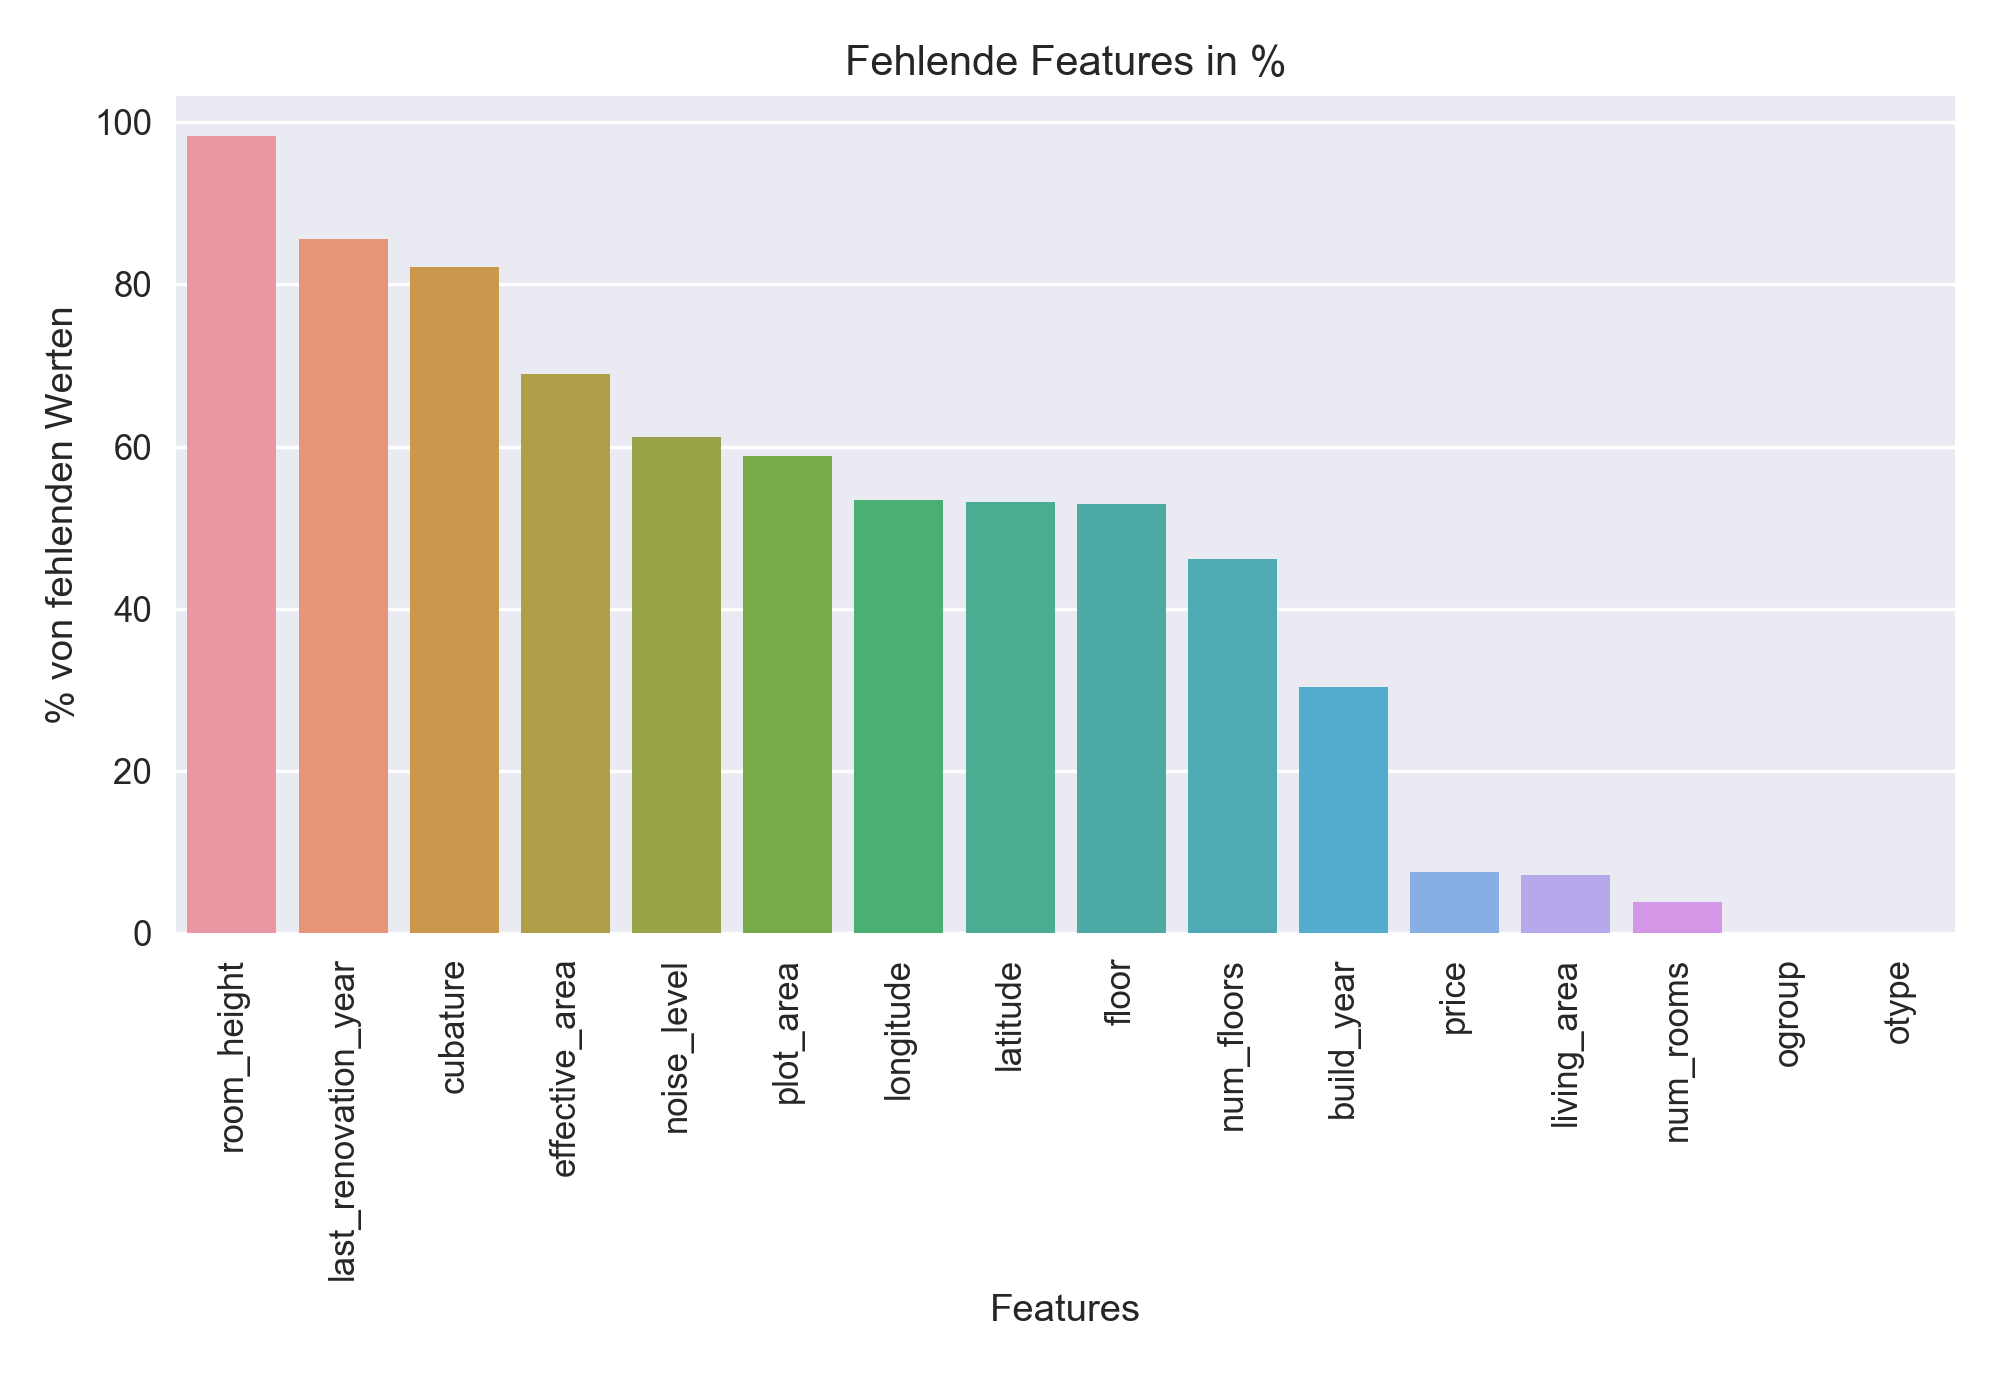
\includegraphics[width=0.9\textwidth]{images/missing_values.png}
\caption[\% Anteil der fehlenden Features]{\% Anteil der fehlenden Features}%
\label{fig:features}
\end{figure}
\newline
%
Die Crawler wurden nie über eine längere Zeit gesperrt. Vereinzelt kam es zu Blockierungen, die jedoch, durch das Starten neuer Proxyinstanzen, umgehen werden konnten. Der Zeitaufwand um ein Portal bei fünf gleichzeitigen Verbindungen und einer Downloaddelay von zwei Sekunden zu crawlen, lag im Schnitt bei 4 Stunden. Dementsprechend wurden in dieser Zeit etwa 100 Proxyinstanzen gestartet.\\[2ex]
%
Die Datenqualität der gesammelten Inserate ist eher mässig, da viele erst gar nicht für ein Trainingsdatensatz verwendet werden können. Um dem entgegenzuwirken, wurde versucht durch Feature Engineering fehlende Daten zu berechnen.
%
\subsubsection{Kaufpreis}
Abbildung \ref{fig:price} zeigt die Verteilung des Kaufpreises. Abbildung \ref{fig:verteilung_price_all} beinhaltet alle Inserate wobei Abbildung \ref{fig:verteilung_price_part} nur einen Ausschnitt anzeigt. Dabei sieht man, dass der Preis nicht normalverteilt ist. Es besteht eine positive Skenwess, was für eine Lineare Regression nicht optimal ist.\\
Die meisten Inserate besitzen einen Preis zwischen 0 CHF und 2'000'000 CHF. Das Preisspektrum ist ausser ein paar Ausreisser nicht stark verstreut. 
Tabelle \ref{tab:price} zeigt die beschreibenden statistischen Werte des Kaufpreises. Es ist zu sehen, dass die Standardabweichung von Wohnungen fast halb so klein ist, wie die der Häuser. Das liegt unter anderem daran, dass Wohnungspreise kein so grosses Preisspektrum besitzen.
%
\begin{figure}[ht]
\begin{subfigure}{.5\textwidth}
  \centering
  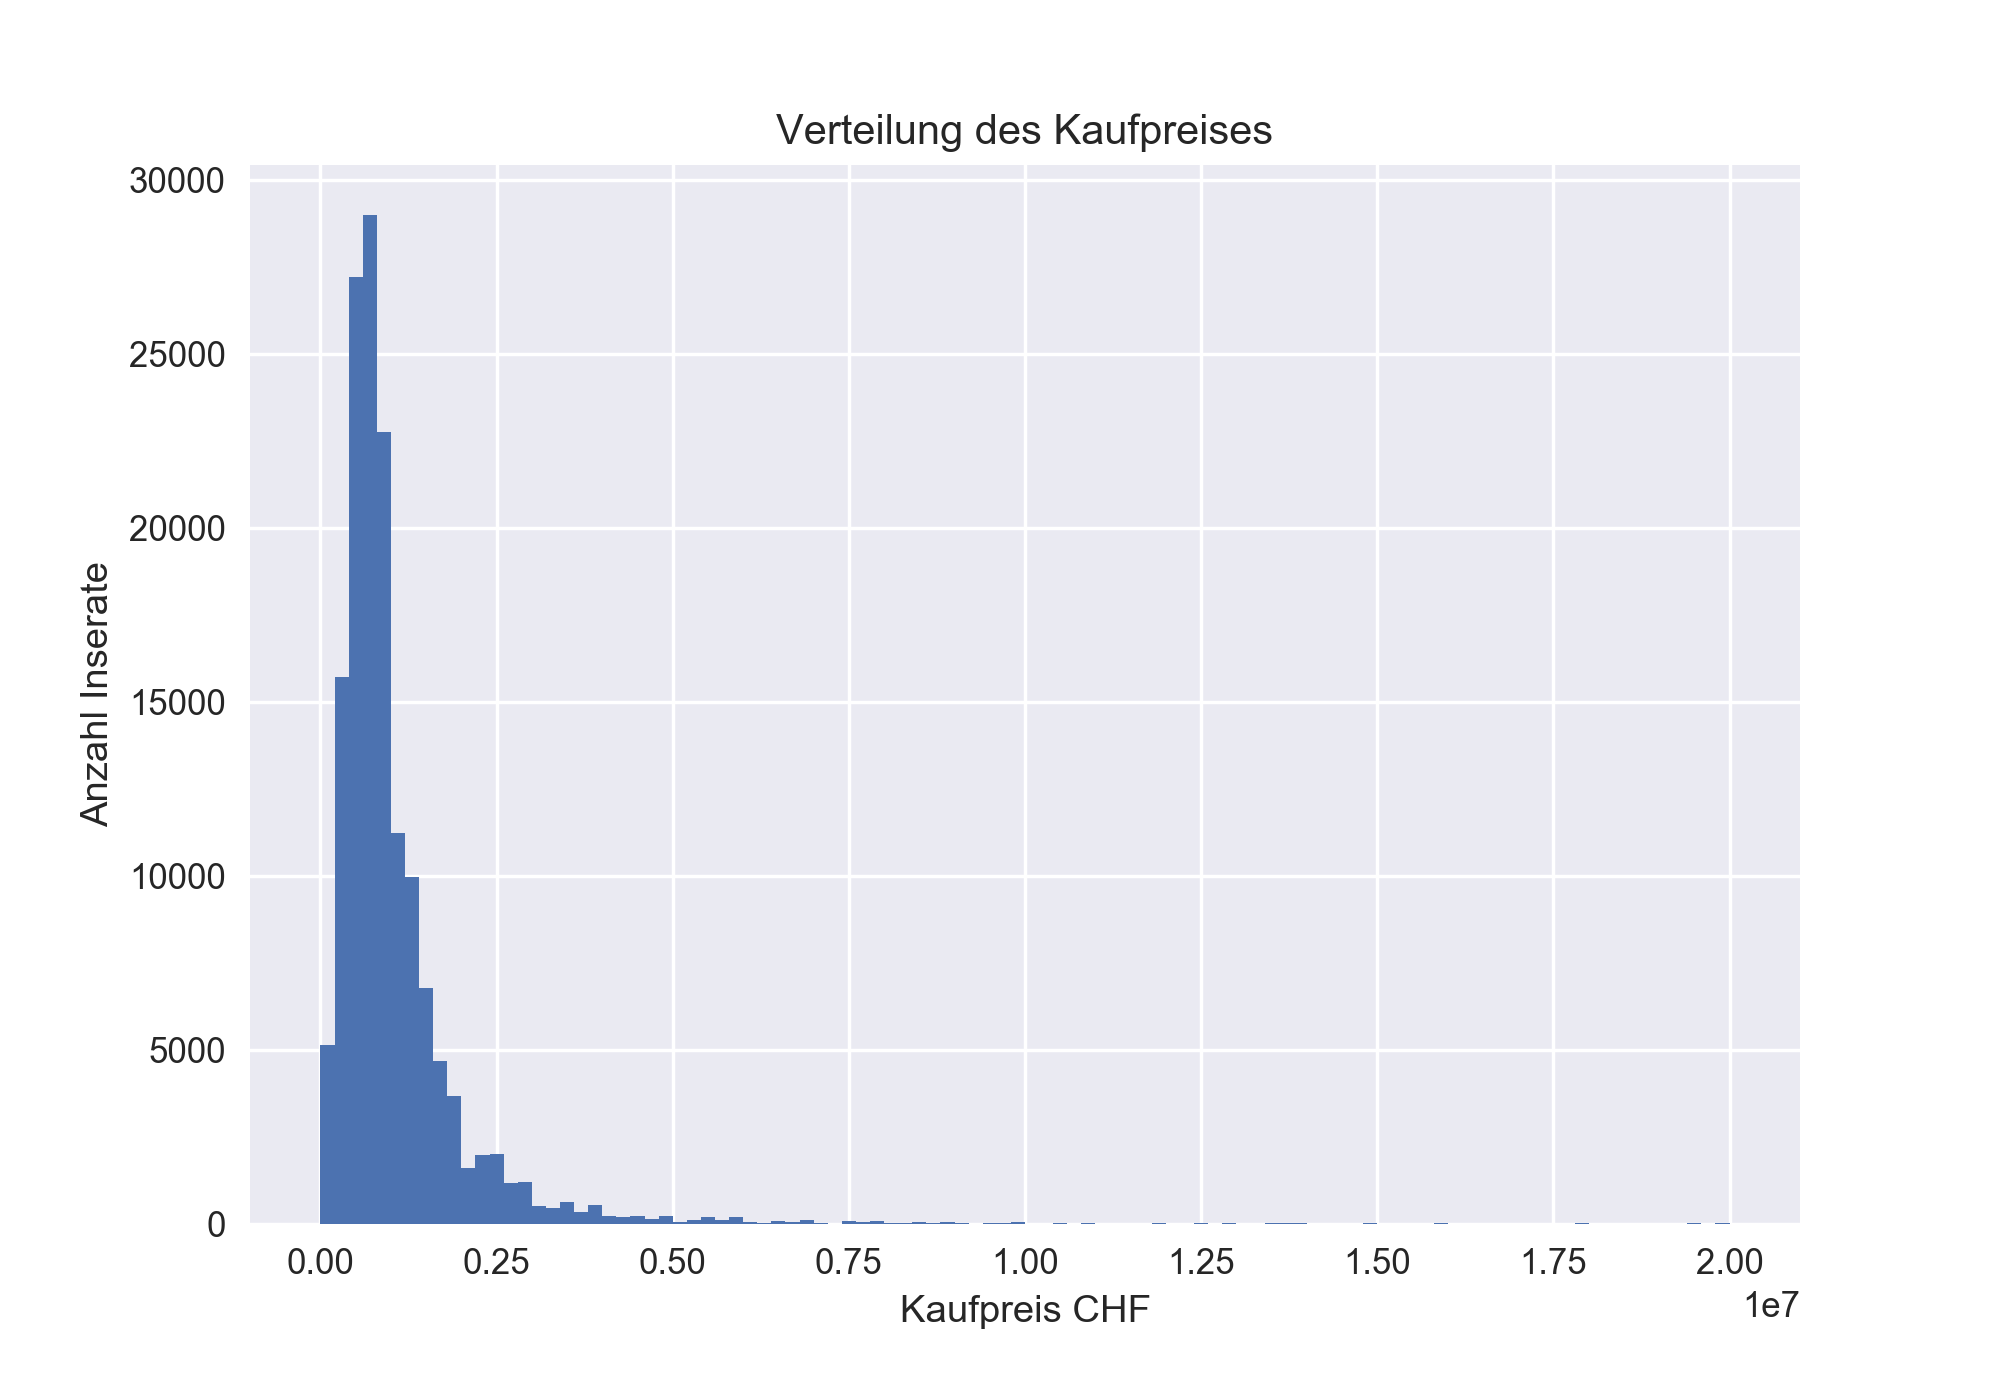
\includegraphics[width=\linewidth]{images/bar_des_kauf_preises.png}
  \caption[Verteilung des Preises mit allen Daten]{Verteilung des Preises mit allen Daten}
  \label{fig:verteilung_price_all}
\end{subfigure}%
\begin{subfigure}{.5\textwidth}
  \centering
  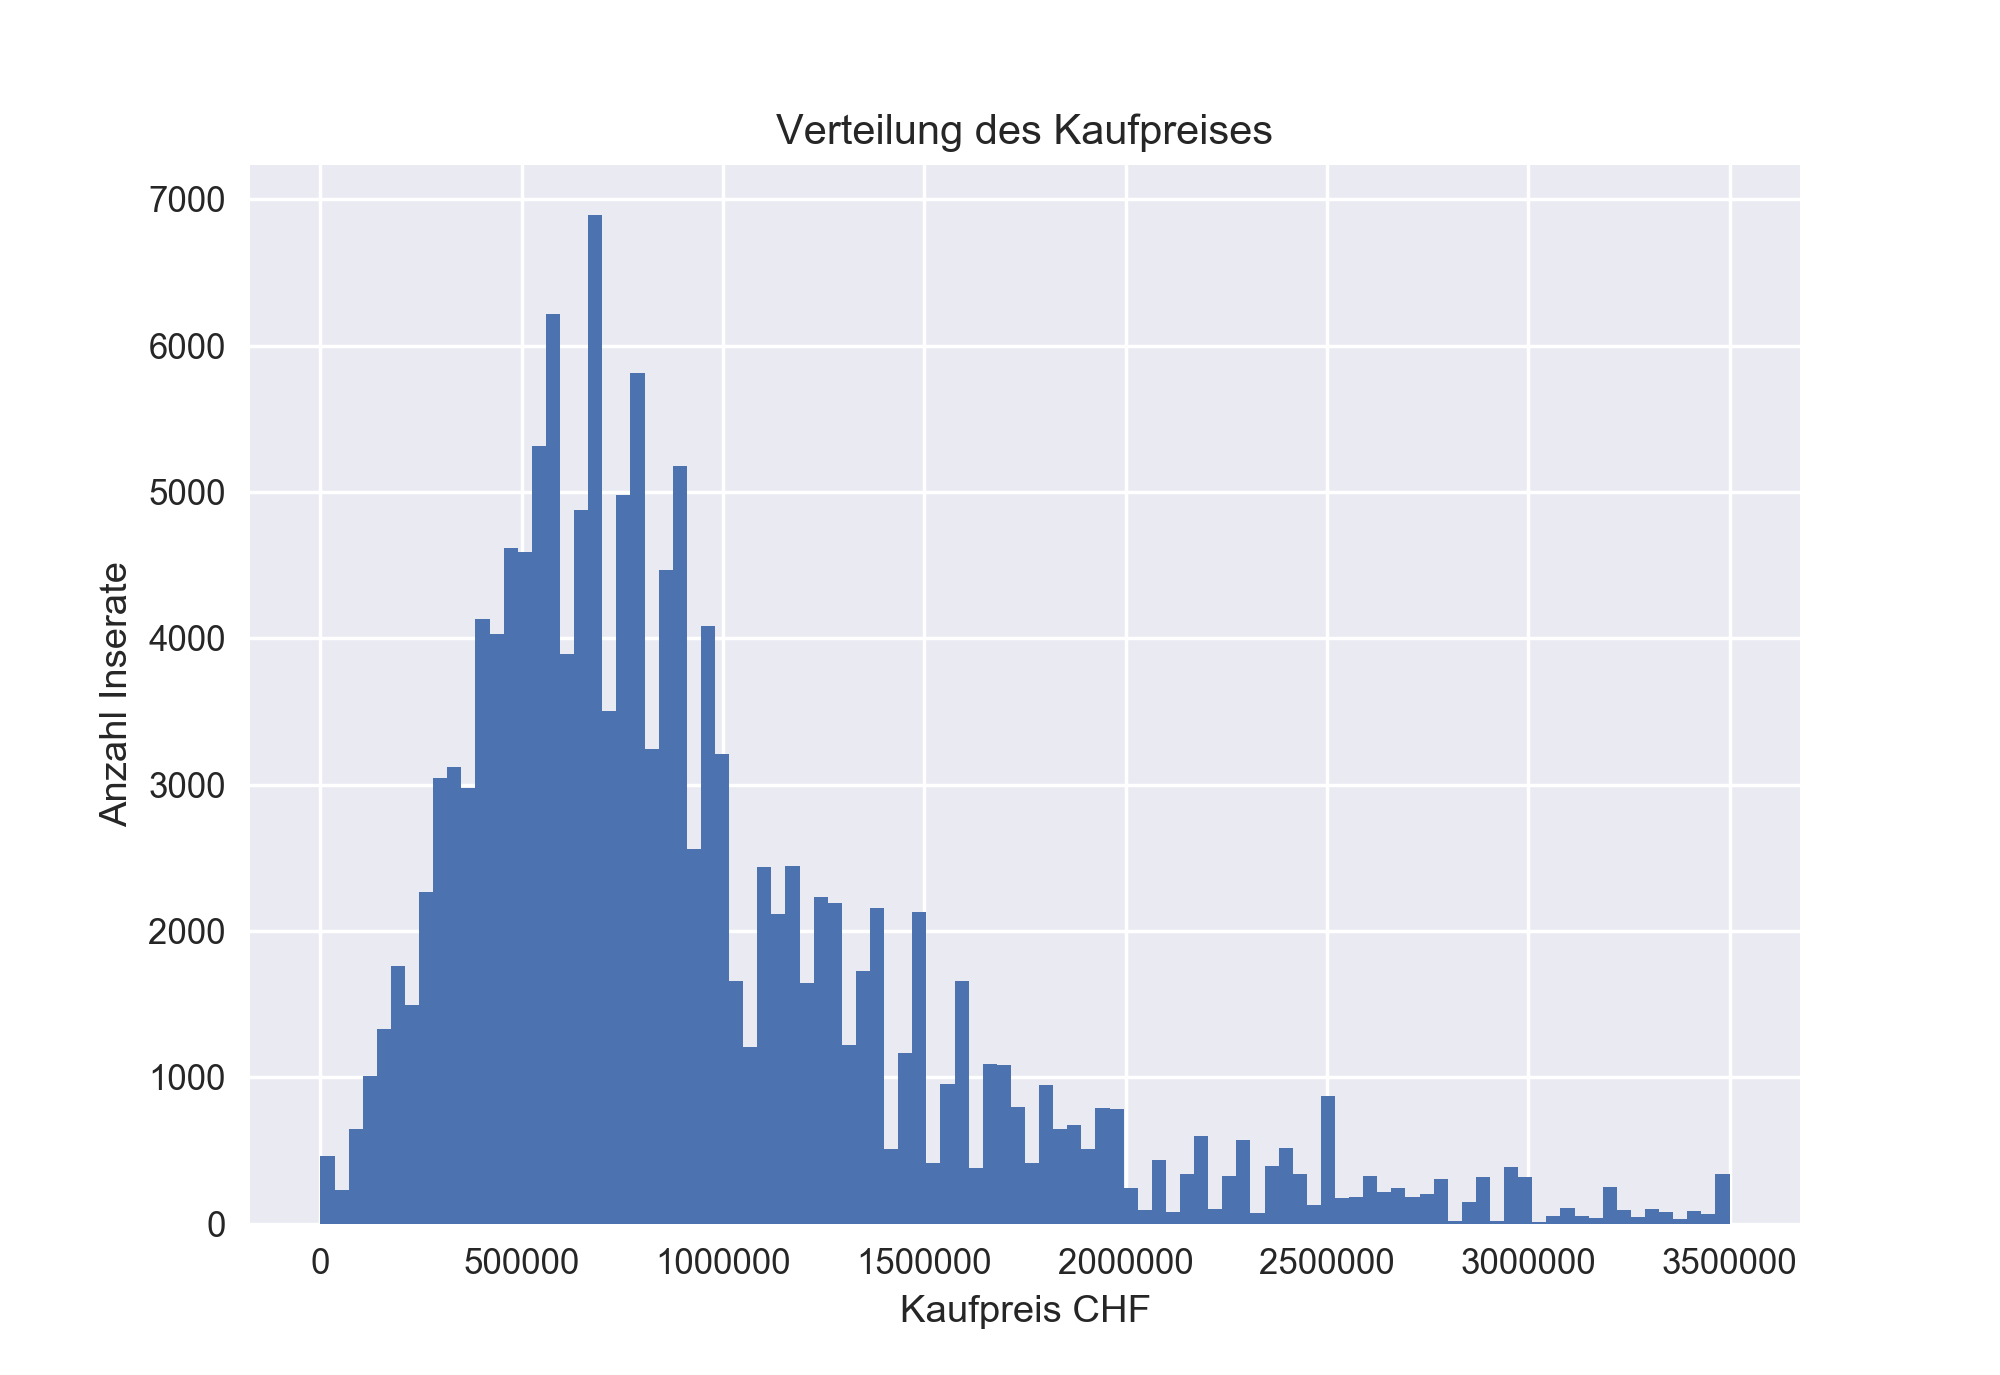
\includegraphics[width=\linewidth]{images/bar_des_kauf_preises_cut.png}
  \caption[Verteilung des Preises von 0 CHF - 2.5 Mio CHF]{Verteilung des Preises von 0 CHF - 2.5 Mio CHF}
  \label{fig:verteilung_price_part}
\end{subfigure}
\caption[Vereilung des Kaufpreises]{Vereilung des Kaufpreises}
\label{fig:price}
\end{figure}
%
\begin{table*}[ht]
\centering
\ra{1.3}
\resizebox{\textwidth}{!}{
\begin{tabular}{@{}lrrrrr@{}}
\toprule
Objektart & Min & Max & Durchschnitt & Median & Standardabweichung\\
\midrule
Wohnung & 10 & 20'000'000 & 891’479 & 690’000 & 786’047\\
Haus & 10 & 20'000'000 & 1'281'735 & 920'000 & 1'309'085\\
Wohnung \& Haus & 10 & 20’000'000 & 1’059’503 & 790’000 & 1’066’372\\
\bottomrule
\end{tabular}}
\caption{Statistische Werte des Kaufpreises}
\label{tab:price}
\end{table*}
%
\subsubsection{Numerische Features}
Bis auf die Lärmbelastung wurden alle numerischen Features von den Immobilienportalen gesammelt.\\
Abbildung \ref{fig:num_features} zeigt einen Teil dieser Features in Verbindung zum Kaufpreis. Dabei ist ersichtlich, dass die Wohnfläche, Kubatur und Anzahl Zimmer eine linear ähnliche Abhängigkeit besitzen. Beim Rest ist eher unklar, wie sie zum Preis stehen.\\[2ex]
%
\begin{figure}[ht]
\centering
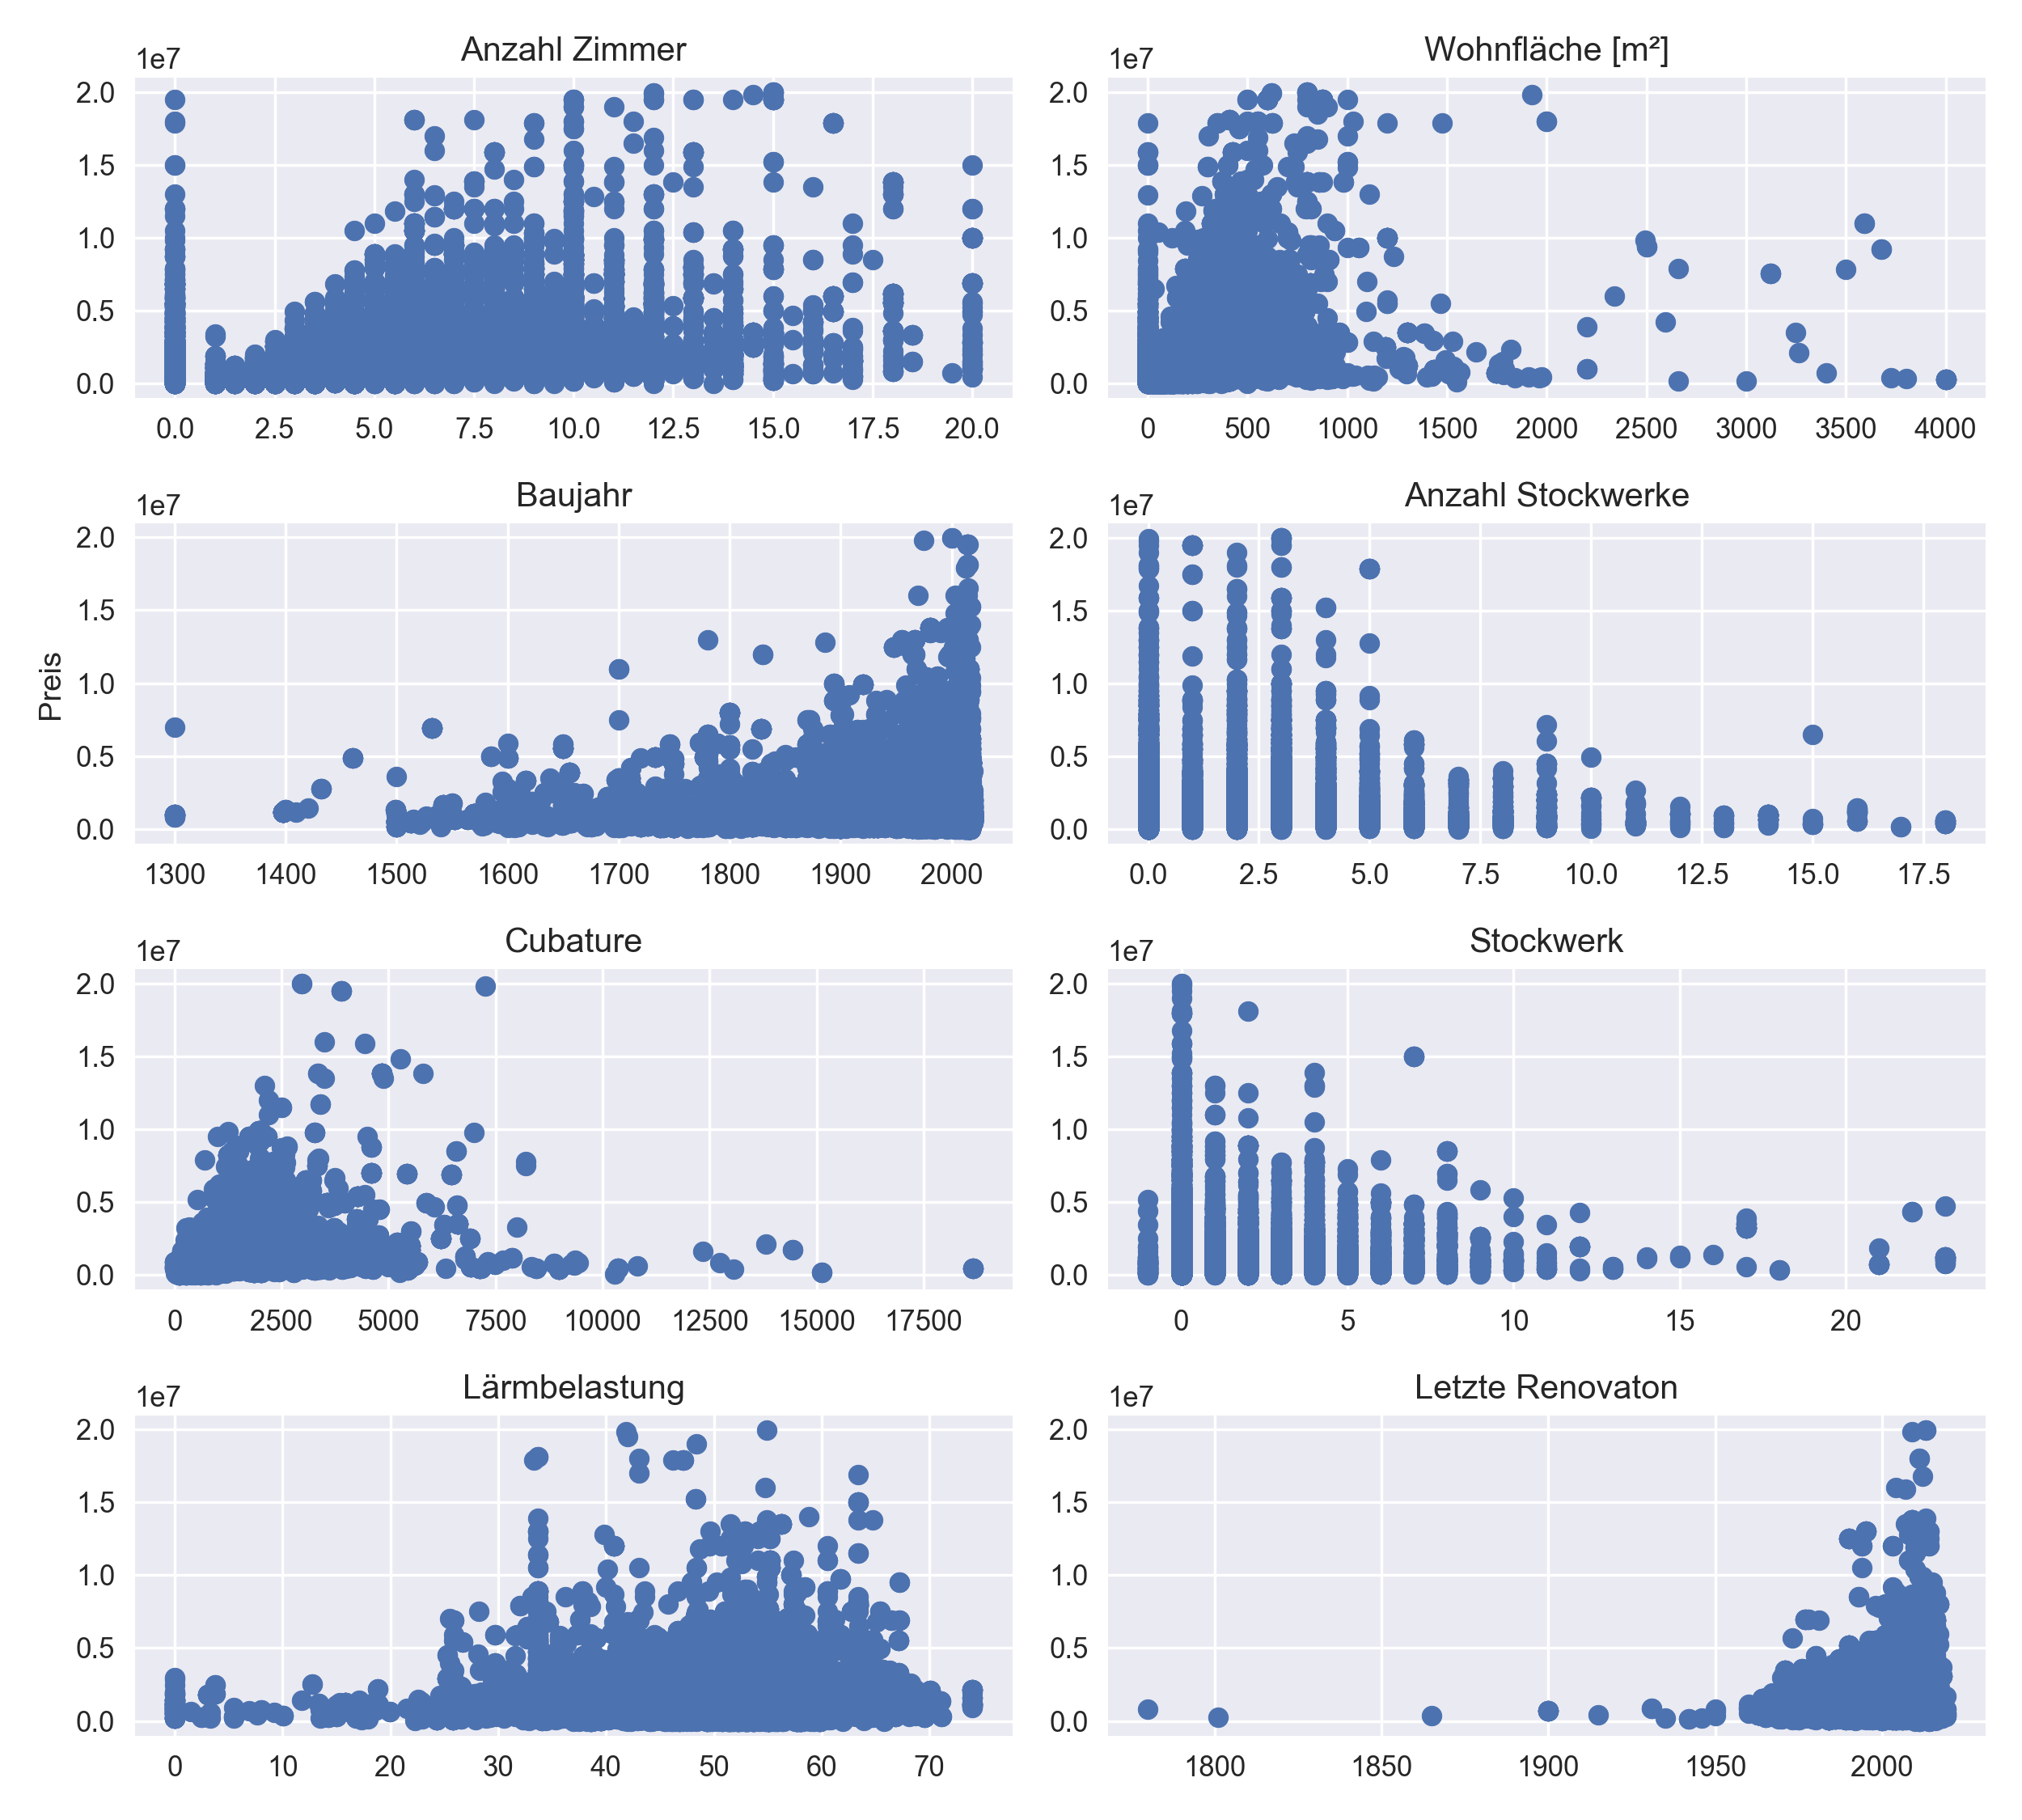
\includegraphics[width=0.9\textwidth]{images/Vergleich_zum_preis.png}
\caption[Nummerische Feature im Vergleich zum Preis]{Nummerische Feature im Vergleich zum Preis}%
\label{fig:num_features}
\end{figure}
\newline
%
Tabelle \ref{tab:num_features} zeigt die statistischen Werte für die numerischen Features. Die gesammelten Kennwerte sehen plausibel aus und decken sich zum Teil mit den Daten vom Bundesamt für Statistik\footnote{https://www.bfs.admin.ch/bfs/de/home/statistiken/bau-wohnungswesen.html}.\\
Auffallend ist, dass der Durchschnitt und der Median bei vielen Features sehr nahe beieinander liegen. Somit gleicht die Verteilung einer Normalverteilung.\\[2ex]
%
\begin{table*}[ht]
\centering
\ra{1.3}
\resizebox{\textwidth}{!}{
\begin{tabular}{@{}lrrrrr@{}}
\toprule
 & Min & Max & Durchschnitt & Median & Standardabweichung\\
\midrule
Anz. Zimmer & 0& 20 & 4.84 & 4.5 & 1.9\\
Fläche & 0 & 4’000 & 143.08 & 130 & 101.924\\
Baujahr & 1300 & 2019 & 1988 & 2006 & 51.52\\
Anz. Stockwerke & 0 & 18 & 1.8 & 2 & 1.747\\
Kubatur & 1 & 18649 & 1059.74 & 867 & 838.419\\
Stockwerk & -1 & 23 & 1.25 & 1 & 1.57\\
Lärmbelastung & 0 & 73.99 & 48.8 & 49.35 & 6.85\\
Letzte Renovation & 1780 & 2019 & 2009 & 2012 & 9.09\\
\bottomrule
\end{tabular}}
\caption{Statistische Werte der nummerischen Features}
\label{tab:num_features}
\end{table*}
%
Abbildung \ref{fig:heatmap} zeigt eine Heatmap der einzelnen Features. Diese zeigt auf, welche Features  untereinander korrelieren. Der Kaufpreis hat die höchste Korrelationen mit der Wohnfläche und der Anzahl Zimmer. Weniger starke Korrelationen besitzt er mit dem Baujahr sowie Stockwerk.
%
\begin{figure}[h!]
\centering
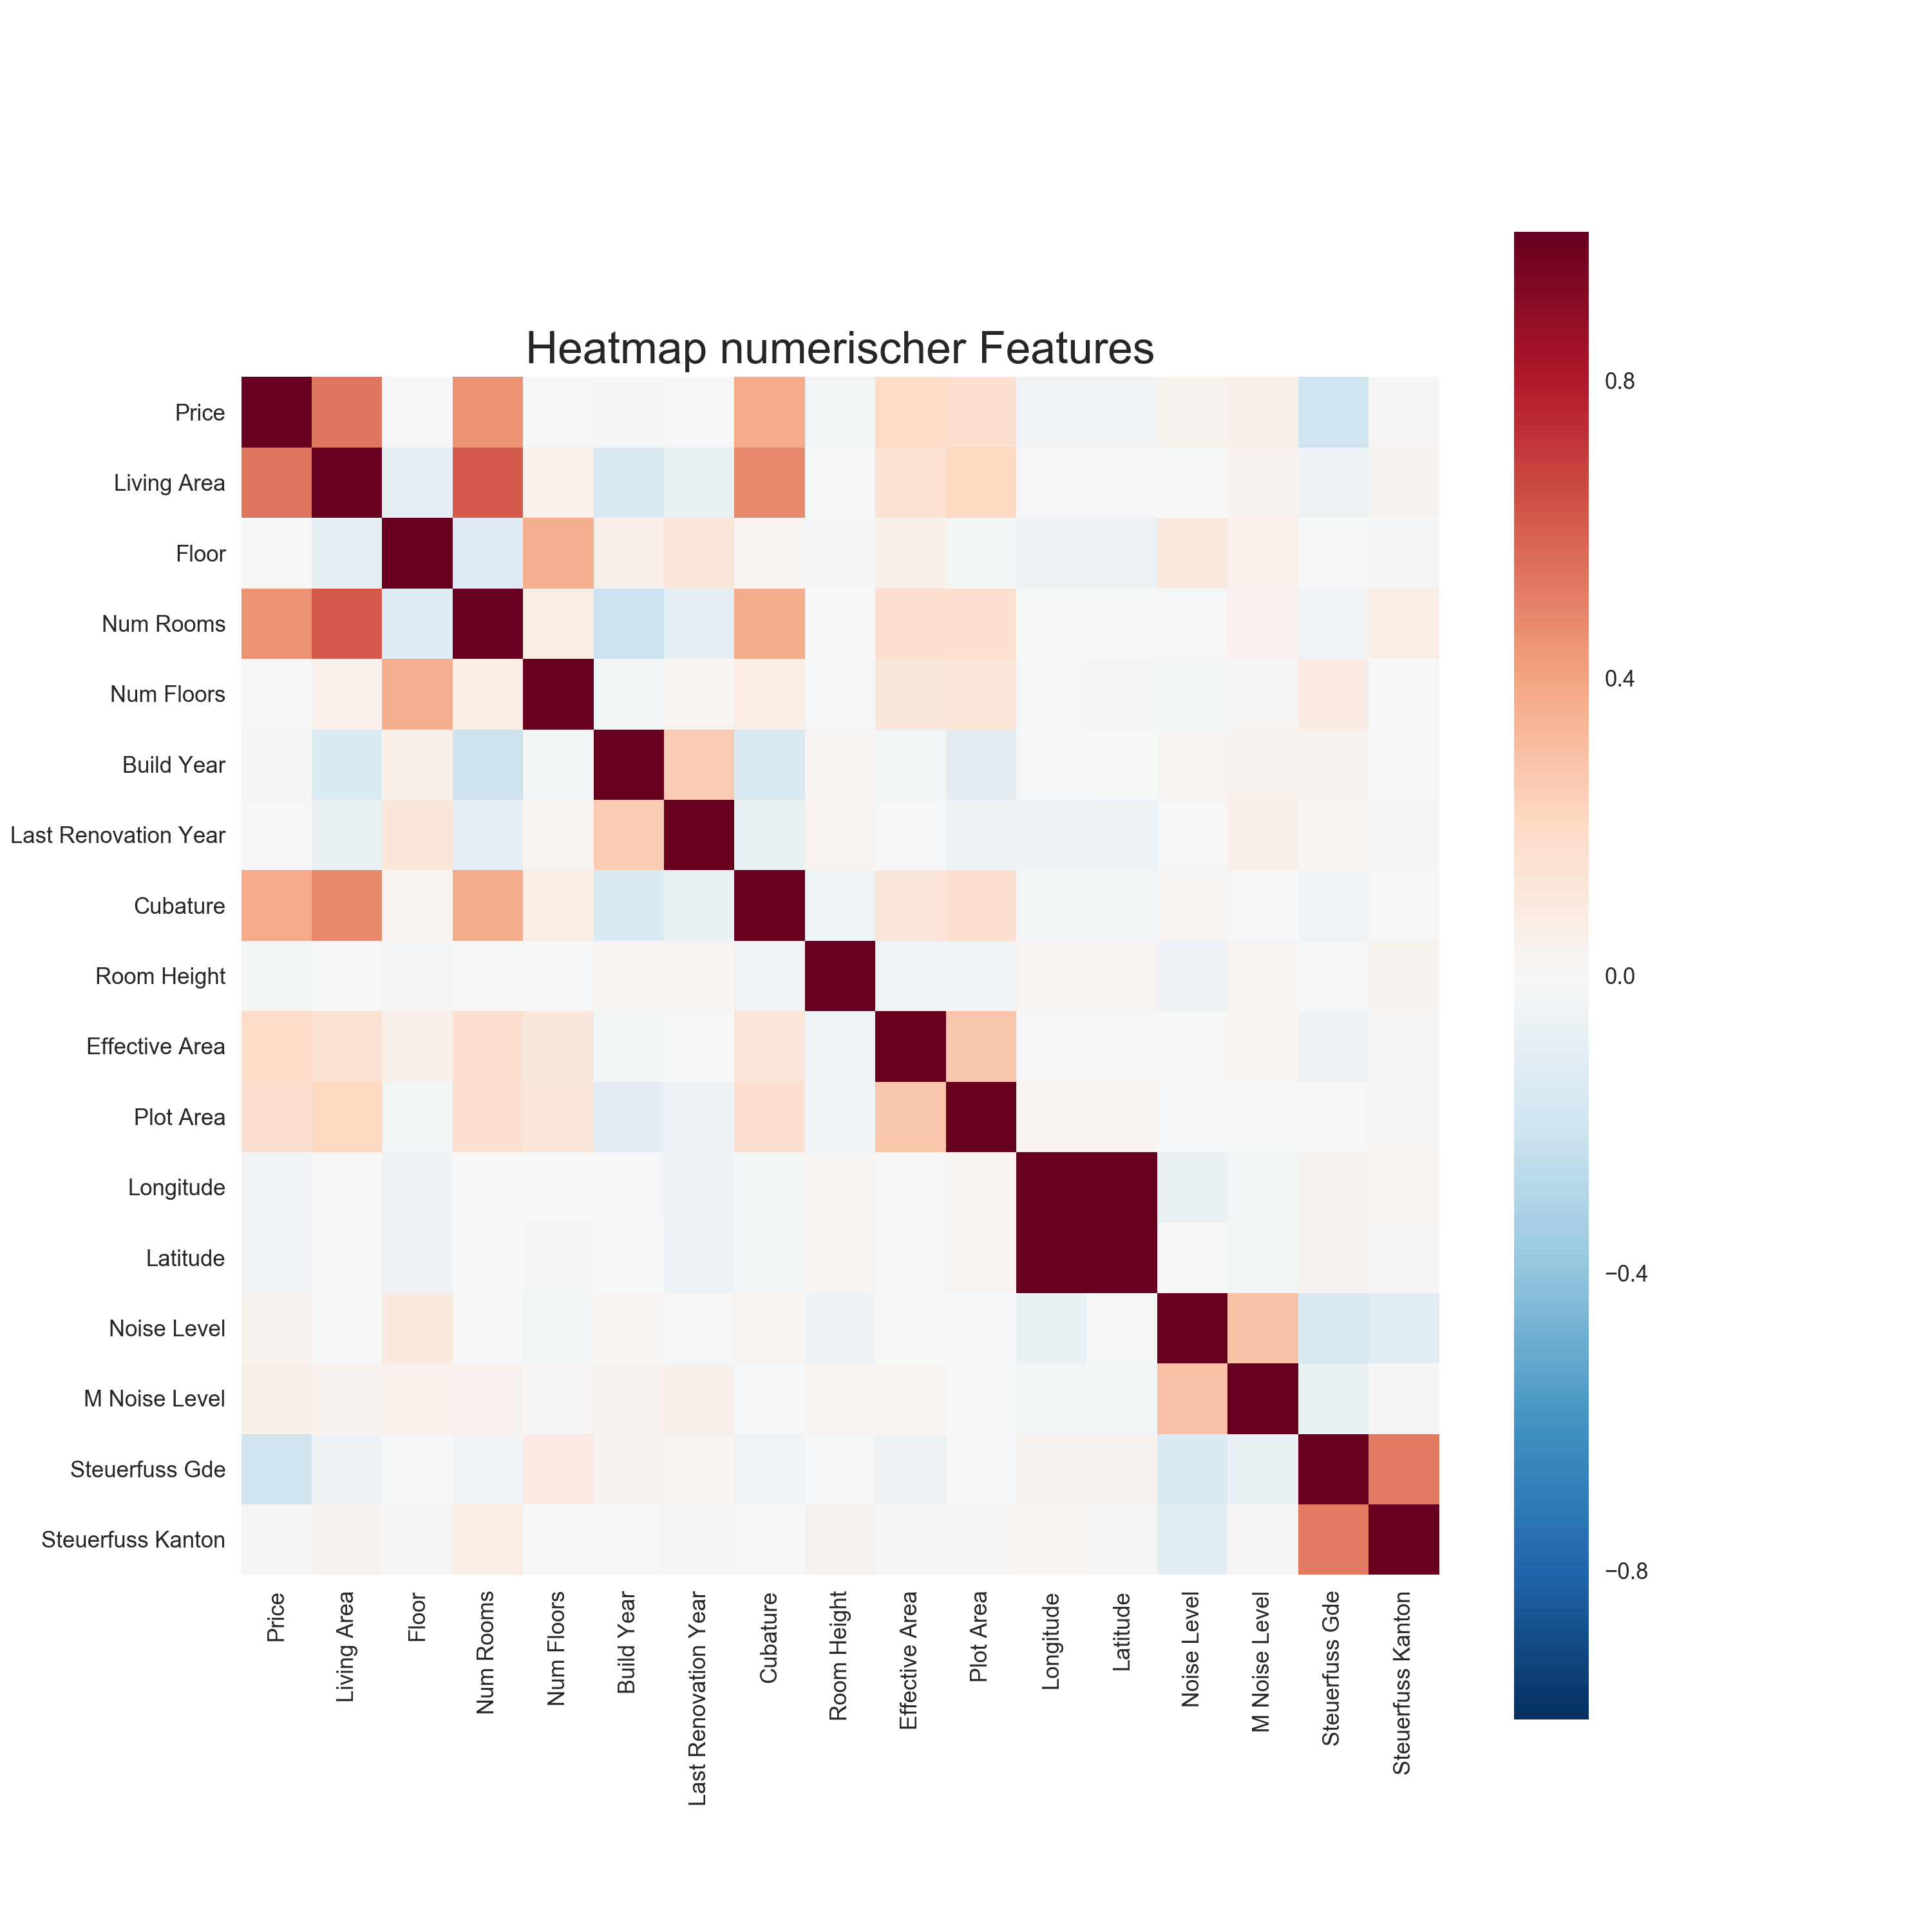
\includegraphics[width=0.9\textwidth]{images/Heatmap_numerical.png}
\caption[Heatmap der nummerischen Features]{Heatmap der nummerischen Features}%
\label{fig:heatmap}
\end{figure}
\newline
%
\subsubsection{Kategorische Features}
Bei den Kategorischen Features handelt es sich vor allem um ortsbezogene Features vom BFS. Viele davon beschreiben die Region, indem sich die Immobilie befindet.\\
Insgesamt wurden 35 kategorische Features verwendet. Eine Analyse der ortsbezogenen Features mit dem Kaufpreis ergab keine unerwarteten Ergebnisse. So zeigt Abbildung \ref{fig:cantons}, dass der Kanton Genf die teuersten Immobilien in der Schweiz besitzt, gefolgt von Zug.
Auch ist ersichtlich, dass städtische Immobilien im Schnitt teurer sind als auf dem Land, beziehungsweise je urbaner die Region, desto teurer der Immobilienpreis. Diverse weitere Vergleiche befinden sich im Anhang.\\[2ex]
\begin{figure}[ht]
\centering
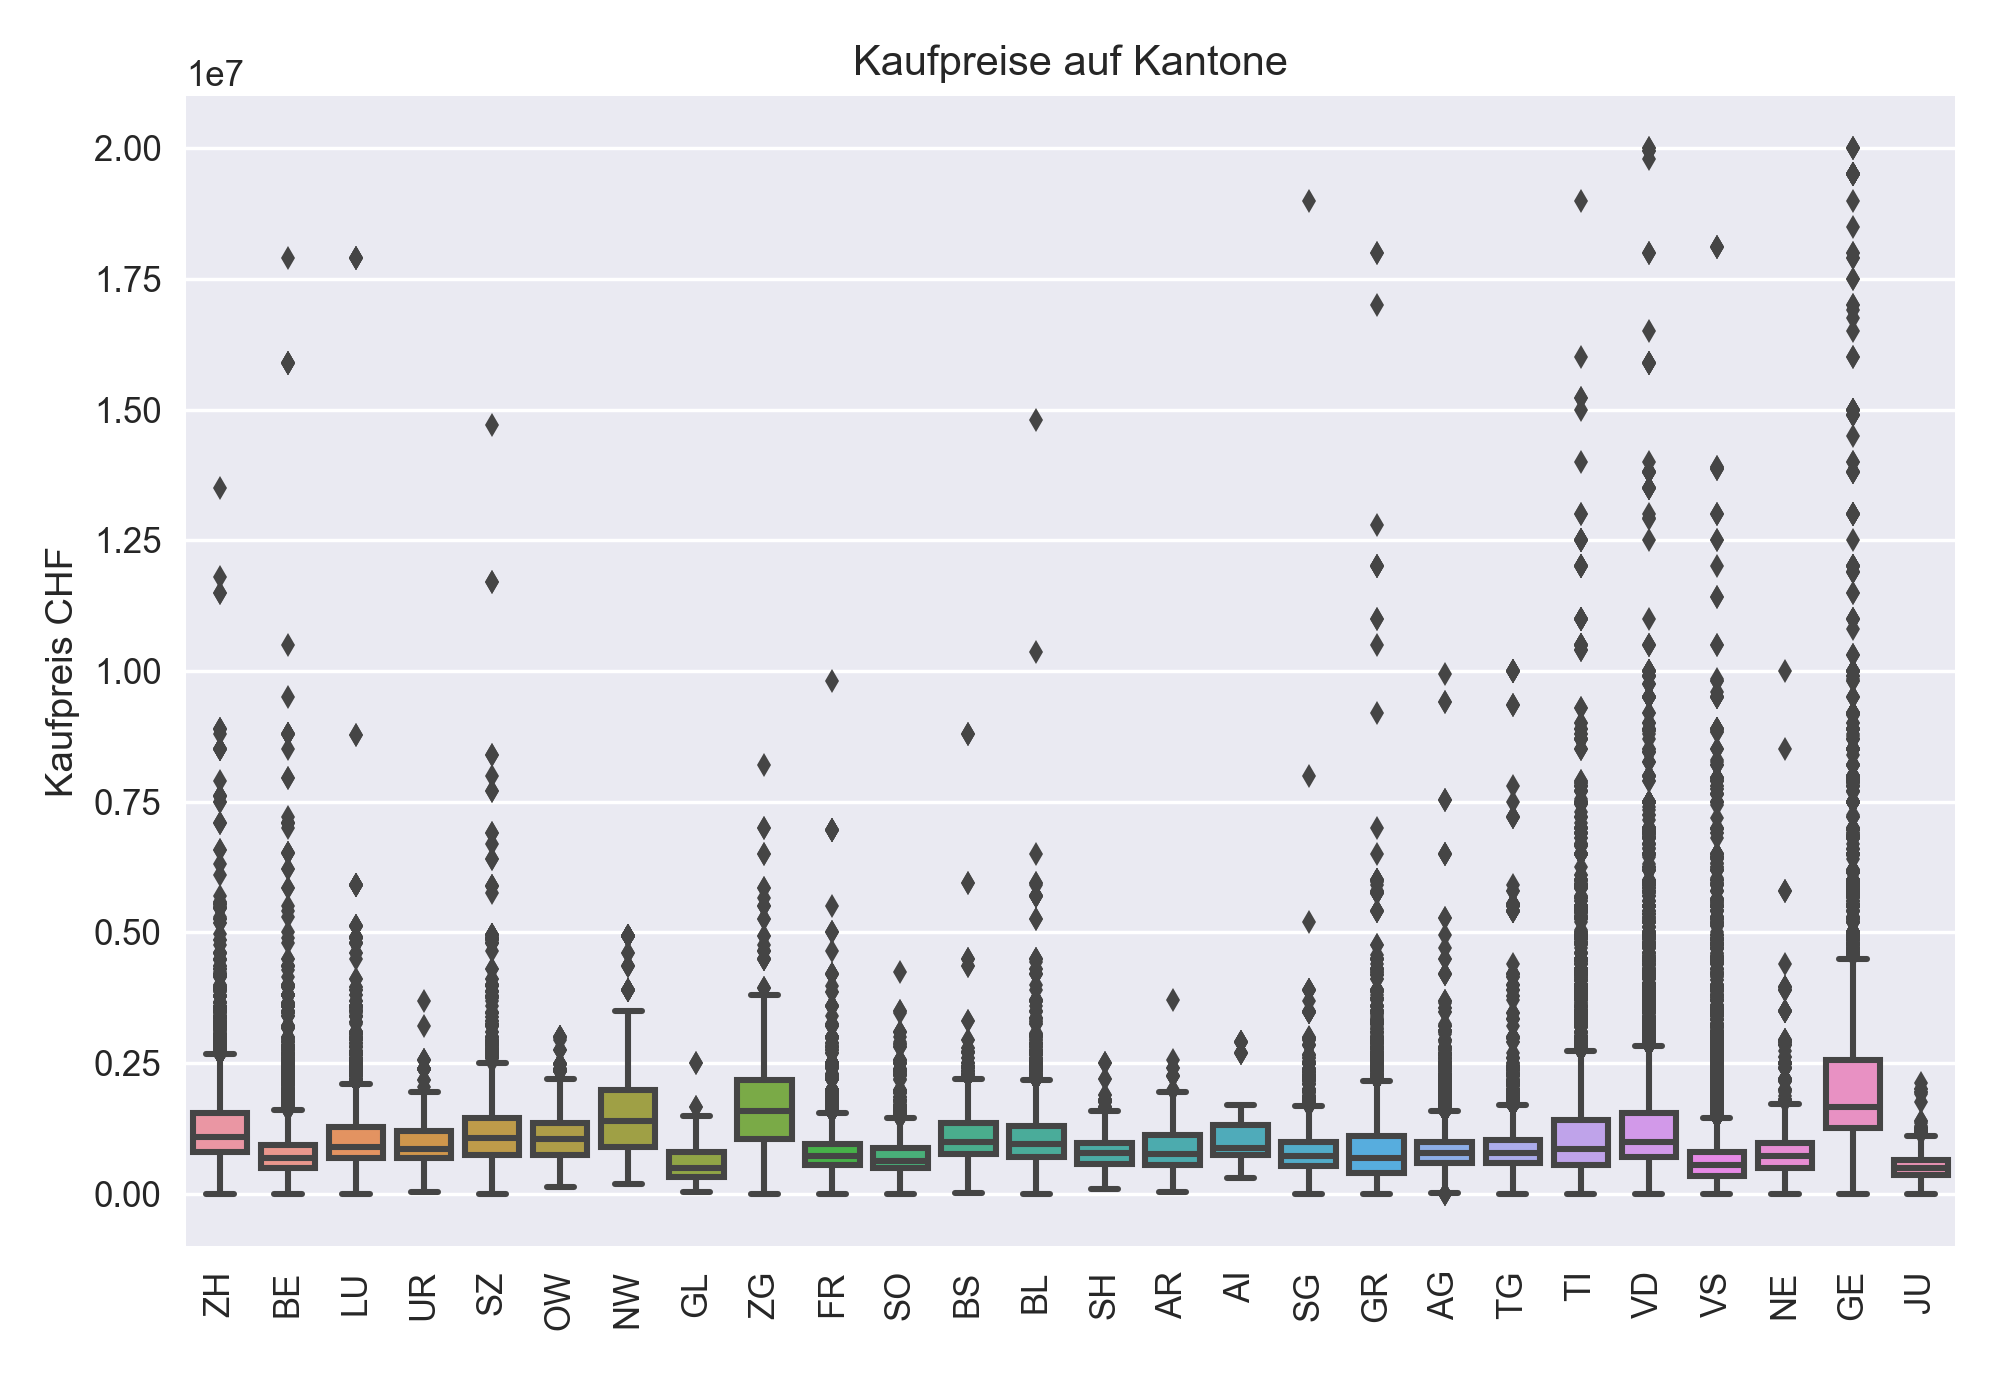
\includegraphics[width=\textwidth]{images/boxPlot_cantons.png}
\caption[Kaufpreis auf Kantonte aufgeteilt]{Kaufpreis auf Kantonte aufgeteilt}%
\label{fig:cantons}
\end{figure}
\newline
%
\textbf{Beschreibung / Merkmale}\\
Neben den ortsbezogenen Daten, analysierten wir die Beschreibung und die Merkmale der Inserate, um verschiedene Tags zuordnen zu können. Die 50 häufigsten vorkommenden Tags die in unserem Datensatz vorkamen, werden in Abbildung \ref{fig:tags} gezeigt. Die verwendeten Tags beschreiben vor allem die Innen- und Ausseneinrichtung einer Immobile.
%
\begin{figure}[ht]
\centering
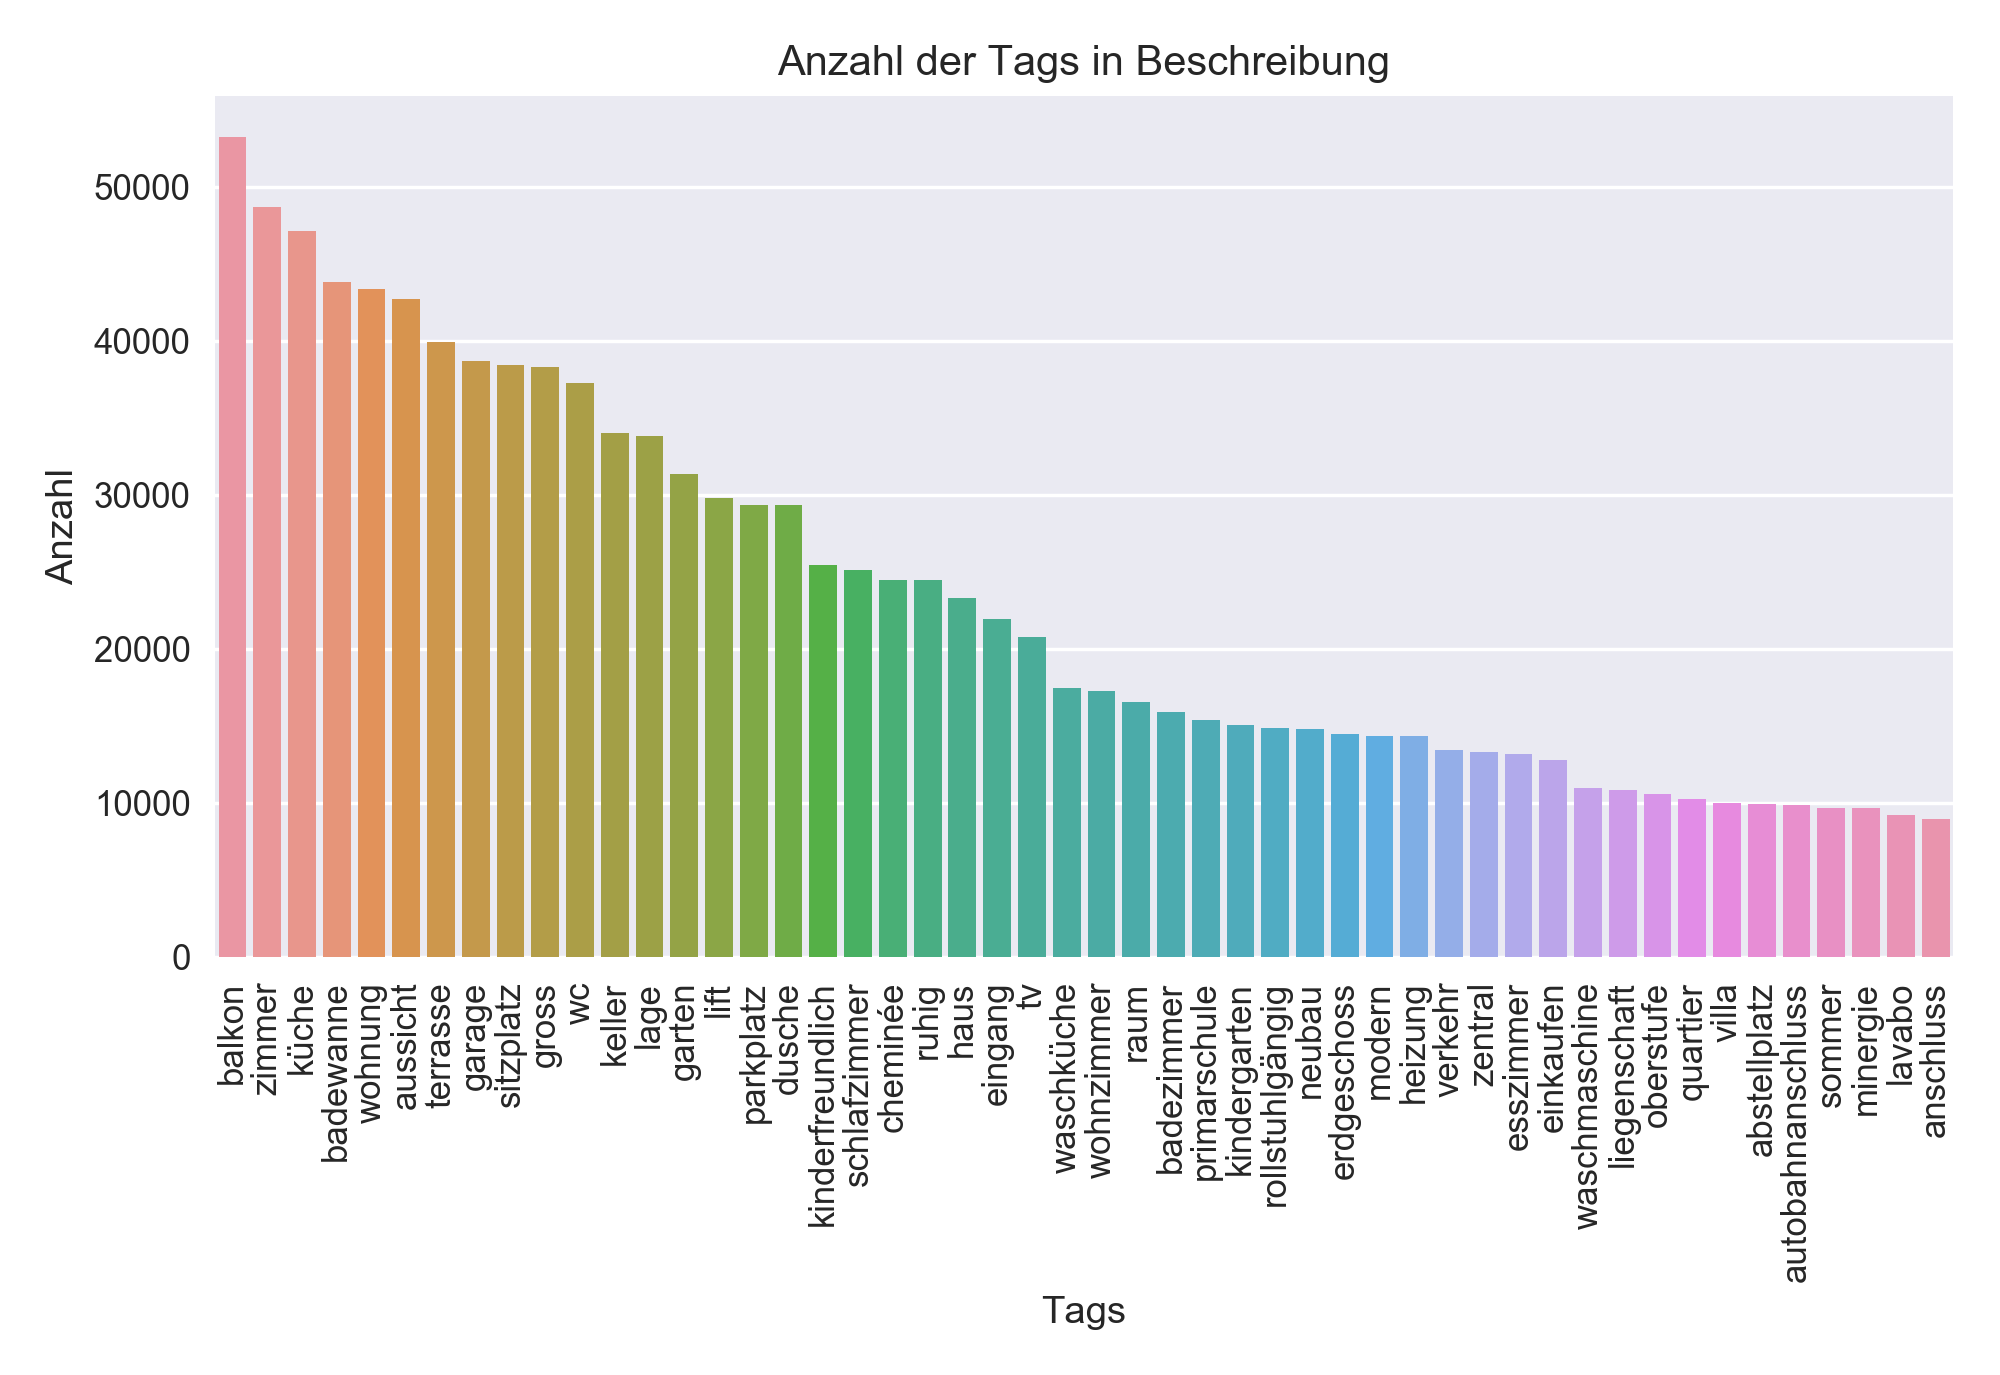
\includegraphics[width=\textwidth]{images/tags.png}
\caption[50 häufigsten vorkommenden Tags]{50 häufigsten vorkommenden Tags}%
\label{fig:tags}
\end{figure}
\newline
%
\subsection{Machine Learning}
Insgesamt haben wir neun verschiedene Machine Learning Algorithmen untersucht. Um eine faire Bewertung zu bekommen, bekamen alle Algorithmen die gleichen Datensätze zum Trainieren und zum Testen. So wurde verhindert, dass ein Algorithmus anhand eines besseren Datensatzes eine bessere Performance erzielte. Nichtsdestotrotz handelt es sich bei Machine Learning um eine nicht exakte Wissenschaft. Die Resultate müssen also mit einer gewissen Vorsicht betrachtet werden.\\[2ex]
%
Als erstes bereiten wir unsere gesammelten Daten für unsere Algorithmen vor. Dafür werden die Features, wenn nötig, richtig transformiert. Dies geschiet im Feature Engineering. In den nächsten Absätzen wird das Feature Engineering sukzessive ergänzt und die Resultate überprüft.\\[2ex]
%
Als Basis für unsere Feature Engineering Pipeline transformieren wir unseren kategorischen Features mit Hilfe einer One-Hot-Encoding in binäre Features um. So enstanden aus 35 Features über 2000 Features.\\
Wie im vorherigen Kapitel gezeigt, sind die Features Kubatur, Raumhöhe, effektive Fläche, Grundstücksfläche, Anzahl Stockwerke, Stockwerk und Renovationsjahr nur selten angegeben. Somit können sie nicht verwendet werden als Features. Dafür können die Wohnfläche, die Anzahl Zimmer, das Baujahr, das Renovationsjahr, die Beschreibung und die Merkmale einer Immobile verwendet werden.\\ 
Als letzter Schritt werden noch die Inserate gelöscht, die keinen Eintrag bei einem verwendeten Feature besitzen oder doppelt vorkommen.
%
\subsubsection{Regressions Algorithmen}
Für die Auswertung der Algorithmen starten wir mit den Regressions Algorithmen. Hierfür verwenden wir eine  einfache lineare Regression, den Ridge- und den Lasso-Algorithmus. Die Ergebnisse werden in Tabelle \ref{tab:regression} angezeigt.\\[2ex]
%
\begin{table*}[ht]
\centering
\ra{1.3}
\resizebox{\textwidth}{!}{
\begin{tabular}{@{}lrrrrr@{}}
\toprule
ML Algorithmus & $R^2$ & MAPE & MdAPE & 10\% Abweichung & Maximaler Fehler\\
\midrule
Lineare Regression & -4.26E+25 & 2.93E+13 & 21.79 & 25.03 & 5.81E+20\\
Ridge Regression & 0.33 & 61.72 & 28.82 & 19.0 & 2.87E+07\\
Lasso Regression & 0.58 & 70.04 & 19.46 & 27.82 & 2.71E+07\\
\bottomrule
\end{tabular}}
\caption{Ergebnisse der Regression Algorithmen}
\label{tab:regression}
\end{table*}
%
Wir sehen, dass die Algorithmen eher schlecht abschneiden. Zum Einen liegt das daran, dass noch kein richtiges Feature Engineering durchgeführt wurde. Zum Anderen haben wir sehr viele kategorischen Features in unserem Modell. Die lineare Regression erwartet eine Normalverteilung der Features, was bei Kategorischen nicht der Fall ist.\\
Es ist ersichtlich, dass die Algorithmen mit einem Regularisierungsparameter eine deutlich bessere Performance erzielen, als die lineare Regression. Somit ist ein Regularisierungsparameter bei über 2000 Features, der ein Overfit verhindert und somit die Komplexität reduziert, nützlich.\\
Auffallend ist, dass der Lasso Algorithmus eine deutliche bessere Performance als der Ridge Algorithmus vorweist. Dies kann auf ein schlechtes Feature Engineering zurückgeführt werden. Denn der Lasso kann unnötige Features eliminieren, während der Ridge alle Features verwendet.
%
\subsubsection{K-Nearest Neighbour}
Beim nächsten Algorithmus handelt es sich um den K-Nearest Neighbour. Dieser Algorithmus versucht anhand der Nachbarn den Preis zu schätzen. Der Vorteil gegenüber den Regressions Algorithmen ist, dass es dem Algorithmus egal ist, in welchem Format die Features sind. Zudem haben viele Features keinen negativen Einfluss auf den Algorithmus.
Tabelle \ref{tab:kneighbour} zeigt die erzielten Resultate des Algorithmus, der zwei Nachbarn zum Vergleich verwendete und eine Leaf size von 100 hatte. Für die Gewichtung wurde die Euklid-Distanz genommen.\\[2ex]
%
\begin{table*}[ht]
\centering
\ra{1.3}
\resizebox{\textwidth}{!}{
\begin{tabular}{@{}lrrrrr@{}}
\toprule
ML Algorithmus & $R^2$ & MAPE & MdAPE & 10\% Abweichung & Maximaler Fehler\\
\midrule
K-Nearest Neighbour & 0.83 & 23.67 & 0 & 79.94 & 1.81E+07\\
\bottomrule
\end{tabular}}
\caption{Ergebnisse vom K-Nearest Neighbour}
\label{tab:regression}
\end{table*}
%
Die Performance ist deutlich besser als bei den Regressions Algorithmen. 79,94\% der Immobilien können mit einer Abweichung von 10\% richtig geschätzt werden. Anhand diesen Ergebnissen kann aufgezeigt werden, dass bei ähnlichen Immobilien auch ein ähnlicher Preis existiert.\\
Eine MdAPE von 0 erklären wir damit, dass es sehr ähnliche Häuser gibt, die den selben Preis besitzen. Wir gehen im Kapitel 5 nochmals genauer darauf ein. Die MAPE mit einem Wert von 23,67\% ist zu hoch, um von einem guten Modell zu sprechen.\\[2ex]
%
\subsubsection{Baum Algorithmen}
Als nächstes untersuchen wir verschiedene Baum-Algorithmen. Baum Algorithmen erfreuen sich aktuell einer grosser Beliebtheit bei diversen Machine Learning Wettbewerben\footnote{https://www.kaggle.com/c/house-prices-advanced-regression-techniques}.\\[2ex]
%
Wir haben uns vier verschiedene Algorithmen ausgesucht. Sie unterscheiden sich hauptsächlich in ihrer Strategie. Der Random Forest wendet eine Art Bagging an. Der XGBoost wie auch der AdaBoost verwenden eine Boostingstrategie und der Extra Trees verwendet weder ein Boosting noch ein Bagging.\\
Für den Random Forest verwendeten wir bis auf die 700 Schätzungsmodelle die Default Parameter. Dasselbe gilt auch für den Extra Trees Algorithmus.\\
Für den AdaBoost haben wir als Basis Schätzungsmodell den DecisionTreeRegressor mit 18 Schätzungsmodelle genommen.\\
Der XGBoost besitzte eine maximale Tiefe von 100 mit einer Lernrate von 0.1 und 350 Schätzungsmodelle.
Die Resultate werden in Tabelle \ref{tab:first_round} dargestellt.\\[2ex]
%
\begin{table*}[ht]
\centering
\ra{1.3}
\resizebox{\textwidth}{!}{
\begin{tabular}{@{}lrrrrr@{}}
\toprule
ML Algorithmus & $R^2$ & MAPE & MdAPE & 10\% Abweichung & Maximaler Fehler\\
\midrule
Random Forest & 0.907 & 23.318 & 2.43 & 77.523 & 1.26E+07\\	
Extra Trees & 0.91 & 23.884 & 0.861 & 81.735 & 1.04E+07\\
XGBoost & 0.898 & 18.712 & 0.809 & 82.014 & 1.46E+07\\
AdaBoost & 0.907 & 18.138 & 0 & 83.692 & 1.63E+07\\
\bottomrule
\end{tabular}}
\caption{Ergebnisse der Baum Algorithmen}
\label{tab:first_round}
\end{table*}
%
Man sieht, dass die Baum Algorithmen, bis auf den Random Forest, eine noch besser Performance haben, als der K-nearest Neighbour. Die vielen kategorischen Features helfen den Baumalgorithmen eine gute Performance zu erzielen. Wie beim K-Nearest Neighbour ist die MAPE zu hoch, um von einem guten Modell zu sprechen.\\[2ex]
%
Für das weitere Vorgehen werden nur noch der Extra Trees, XGBoost und der AdaBoost verwendet, da diese die besten Werte erreichten.\\[2ex]
%
Um eine bessere Performance zu erhalten, wird anhand von Feature Engineering versucht weitere Features zu generieren. Aus den beiden Features Wohnfläche und Anzahl Zimmer, berechnen wir die durchschnittliche Zimmergrösse. Wir nehmen diese beiden Features, da diese eine hohe Korrelation mit dem Preis besitzen. Tabelle \ref{tab:second_round} zeigt die Ergebnisse.\\[2ex]
%
\begin{table*}[ht]
\centering
\ra{1.3}
\resizebox{\textwidth}{!}{
\begin{tabular}{@{}lrrrrr@{}}
\toprule
ML Algorithmus & $R^2$ & MAPE & MdAPE & 10\% Abweichung & Maximaler Fehler\\
\midrule
Extra Trees & 0.903292 & 27.144 & 0.818 & 81.426 & 1.76E+07\\
XGBoost & 0.887841 & 25.273 & 0.752 & 81.938 & 2.30E+07\\
AdaBoost & 0.884758 & 23.275 & 0 & 83.971 & 2.33E+07\\
\bottomrule
\end{tabular}}
\caption{Ergebnisse mit durchschnittlicher Zimmergrösse}
\label{tab:second_round}
\end{table*}
%
Die MAPE hat als einziger Wert ein paar Prozent eingebüst. Der Rest ist etwa gleich geblieben. Interessanterweise besitzen die Wohnfläche, die Anzahl Zimmer und die durchschnittliche Zimmergrösse eine hohe Gewichtung. Die Gefahr bei stark korrelierenden Features ist, dass sie als ein Feature betrachtet werden. Wird eines der Features verwendet, können die anderen korrelierenden Features an Wichtigkeit verlieren. Da das neue Feature wichtig für die Entscheidungsbäume ist, nehmen wir es für zukünftige Modelle auf.\\[2ex] 
%
Als nächstes ergänzen wir die bestehenden Features durch ein binäres Feature, das auf 1 steht falls eine Renovation durchgeführt wurde und auf 0 steht falls nicht.\\
Zusätzlich um nicht auf das Renovationsjahr zu verzichten, transformieren wir dieses Feature um. Wir nehmen nicht die Jahreszahl, sondern die Differenz vom Renovationjahr bis Heute. Fehlt das Renovationsjahr, wird für die Differenz das Baujahr genommen.\\
Tabelle \ref{tab:third_round} zeigt das Ergebnis der Modelle.\\[2ex]
%
\begin{table*}[ht]
\centering
\ra{1.3}
\resizebox{\textwidth}{!}{
\begin{tabular}{@{}lrrrrr@{}}
\toprule
ML Algorithmus & $R^2$ & MAPE & MdAPE & 10\% Abweichung & Maximaler Fehler\\
\midrule
Extra Trees & 0.915152 & 20.048 & 0.87 & 81.804 & 8.87E+06\\
XGBoost & 0.910506 & 20.191 & 0.802 & 82.113 & 9.19E+06\\
AdaBoost & 0.920327 & 18.484 & 0 & 83.528 & 9.75E+06\\
\bottomrule
\end{tabular}}
\caption{Ergebnisse mit Einbezug der Renovation}
\label{tab:third_round}
\end{table*}
%
Obwohl das Renovationsjahr keine starke Korrelation mit dem Kaufpreis besitzt, konnten diese beiden Features die Performance unserer Modelle verbessern. Zusätzlich konnte der maximale Fehler um einiges verringert werden. Für weitere Modelle wird auch dieses transformation verwendet.\\[2ex]
%
Das Bundesamt für Umwelt stellt die Lärmdatenbank sonBASE\footnote{https://www.bafu.admin.ch/dam/bafu/de/dokumente/laerm/statistik/laerm-berechnungsonbaseermitteltlaermbelastunginderschweiz.pdf} online zur Verfügung. Diese beinhaltet unter anderem den Strassenverkehrslärm für die ganze Schweiz. Da wir für einige Häuser eine exakte Adresse besitzen, können wir anhand den Koordinaten die Lärmbelastung aus der sonBase berechnen.\\
Fehlt die exakte Wohnadresse, nehmen wir die Koordinaten der Gemeinde. Um die Lärmbelastung zu berechnen nehmen wir nicht nur den Wert an einem Punkt sondern berechnen einen Durchschnittswert von 255 Pixel, was etwa einem Radius von 10m entspricht. Abbildung \ref{fig:noise} zeigt einen Ausschnitt der Lärmkarte für eine Berechnung der Lärmbelastung.\\[2ex]
\begin{figure}[ht]
\centering
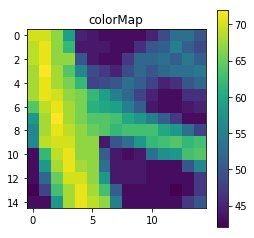
\includegraphics[width=0.5\textwidth]{images/noise.jpeg}
\caption[Ausschnitt der Lärmbelastung am Brausebad (Basel)]{Ausschnitt der Lärmbelastung am Brausebad (Basel)}
\label{fig:noise}
\end{figure}
\newline
%
Tabelle \ref{tab:fourth_round} zeigt die Ergebnisse der Modelle, mit dem neuen Feature Lärmbelastung.\\[2ex]
%
\begin{table*}[ht]
\centering
\ra{1.3}
\resizebox{\textwidth}{!}{
\begin{tabular}{@{}lrrrrr@{}}
\toprule
ML Algorithmus & $R^2$ & MAPE & MdAPE & 10\% Abweichung & Maximaler Fehler\\
\midrule
Extra Trees & 0.838332 & 9.912 & 0.85 & 82.002 & 2.79E+07\\
XGBoost & 0.814466 & 9.952 & 0.74 & 82.212 & 2.81E+07\\
AdaBoost & 0.823295 & 9.954 & 0 & 83.593 & 2.75E+07\\
\bottomrule
\end{tabular}}
\caption{Ergebnisse mit Einbezug der Lärmbelastung}
\label{tab:fourth_round}
\end{table*}
%
Mit hilfe diesen Features konnte die MAPE stark reduziert werden. Da nur nicht bei allen eine exakte Adress vorhanden ist, wird die Lärmbelastung der Gemeinde stärker gewichtet als die exakte.\\[2ex]
%
Auffallend bis jetzt bei allen Modellen war der hohe maximale Fehler zwischen 10 und 25 Millionen. Um diesen Fehler zu verkleinern führen wir vor dem Lernen eine Outlier Detection durch. Somit werden Immobilien mit abnormalen Werten aus dem Datensatz entfernt.\\[2ex]
%
\textbf{Outlier Detection}\\
Für die Outlier Detection verwendeten wir einen Isolation Forest Algorithmus. Es werden nur die numerischen Features auf Ausreisser überprüft, da diese am Fehleranfälligsten sind.\\[2ex]
%
Beim Isolation Forest definiert ein Prozentsatz die Anzahl an markierten Outliers. 
Um einen geeigneten Prozentsatz zu bestimmen, vergleichen wir die entwicklung Standardabweichung bei Erhöhung des Prozentsatz.\\
Ist die Differenz der Standardabweichung mit der Vorherigen nicht um mehr als 2.5\% gesunken, haben wir unseren optimalen Prozentsatz gefunden.\\
Abbildung \ref{fig:outlier} zeigt die Reduktion der Standardabweichung \ref{{fig:isolation_std}} und die gefundenen Outlier \ref{fig:isolation_forest} bei der Wohnfläche. 
%
\begin{figure}[ht]
\begin{subfigure}{.5\textwidth}
  \centering
  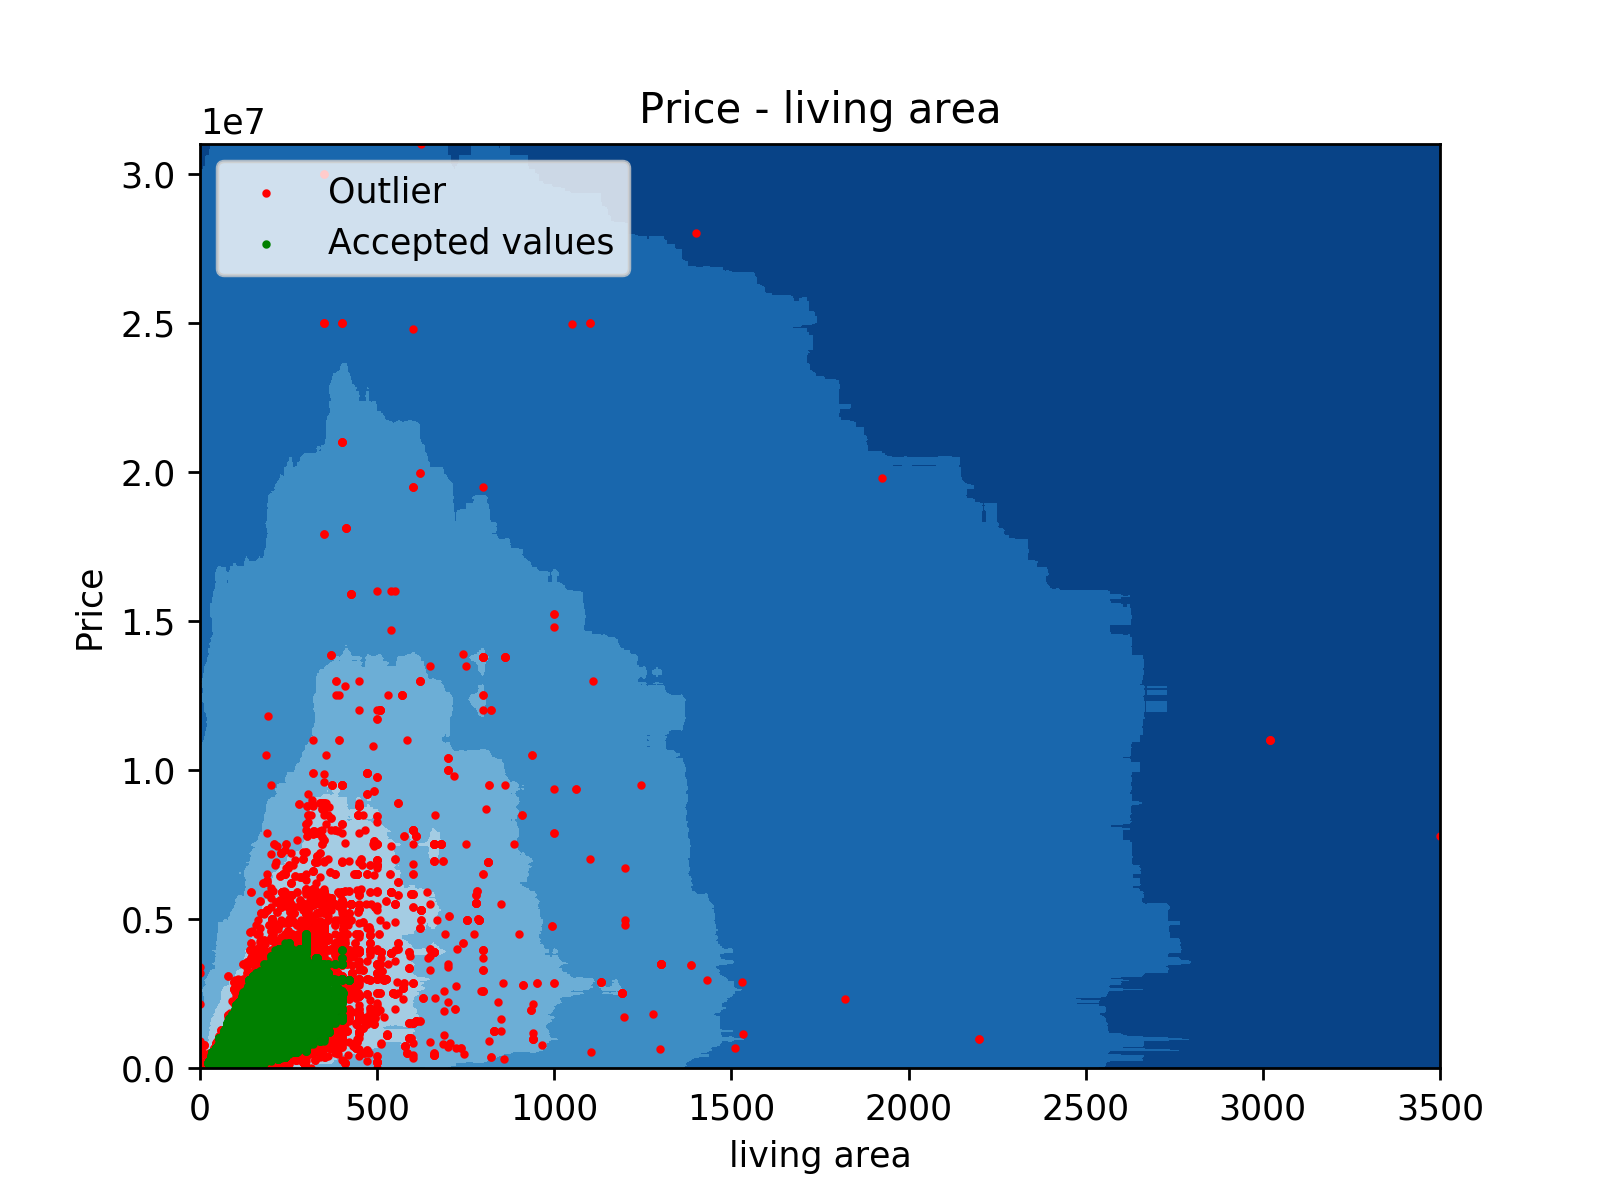
\includegraphics[width=\linewidth]{images/living_area_IsolationForest.png}
  \caption[Isolation Forest angewendet auf Wohnfläche]{Isolation Forest angewendet auf Wohnfläche}
  \label{fig:isolation_forest}
\end{subfigure}%
\begin{subfigure}{.5\textwidth}
  \centering
  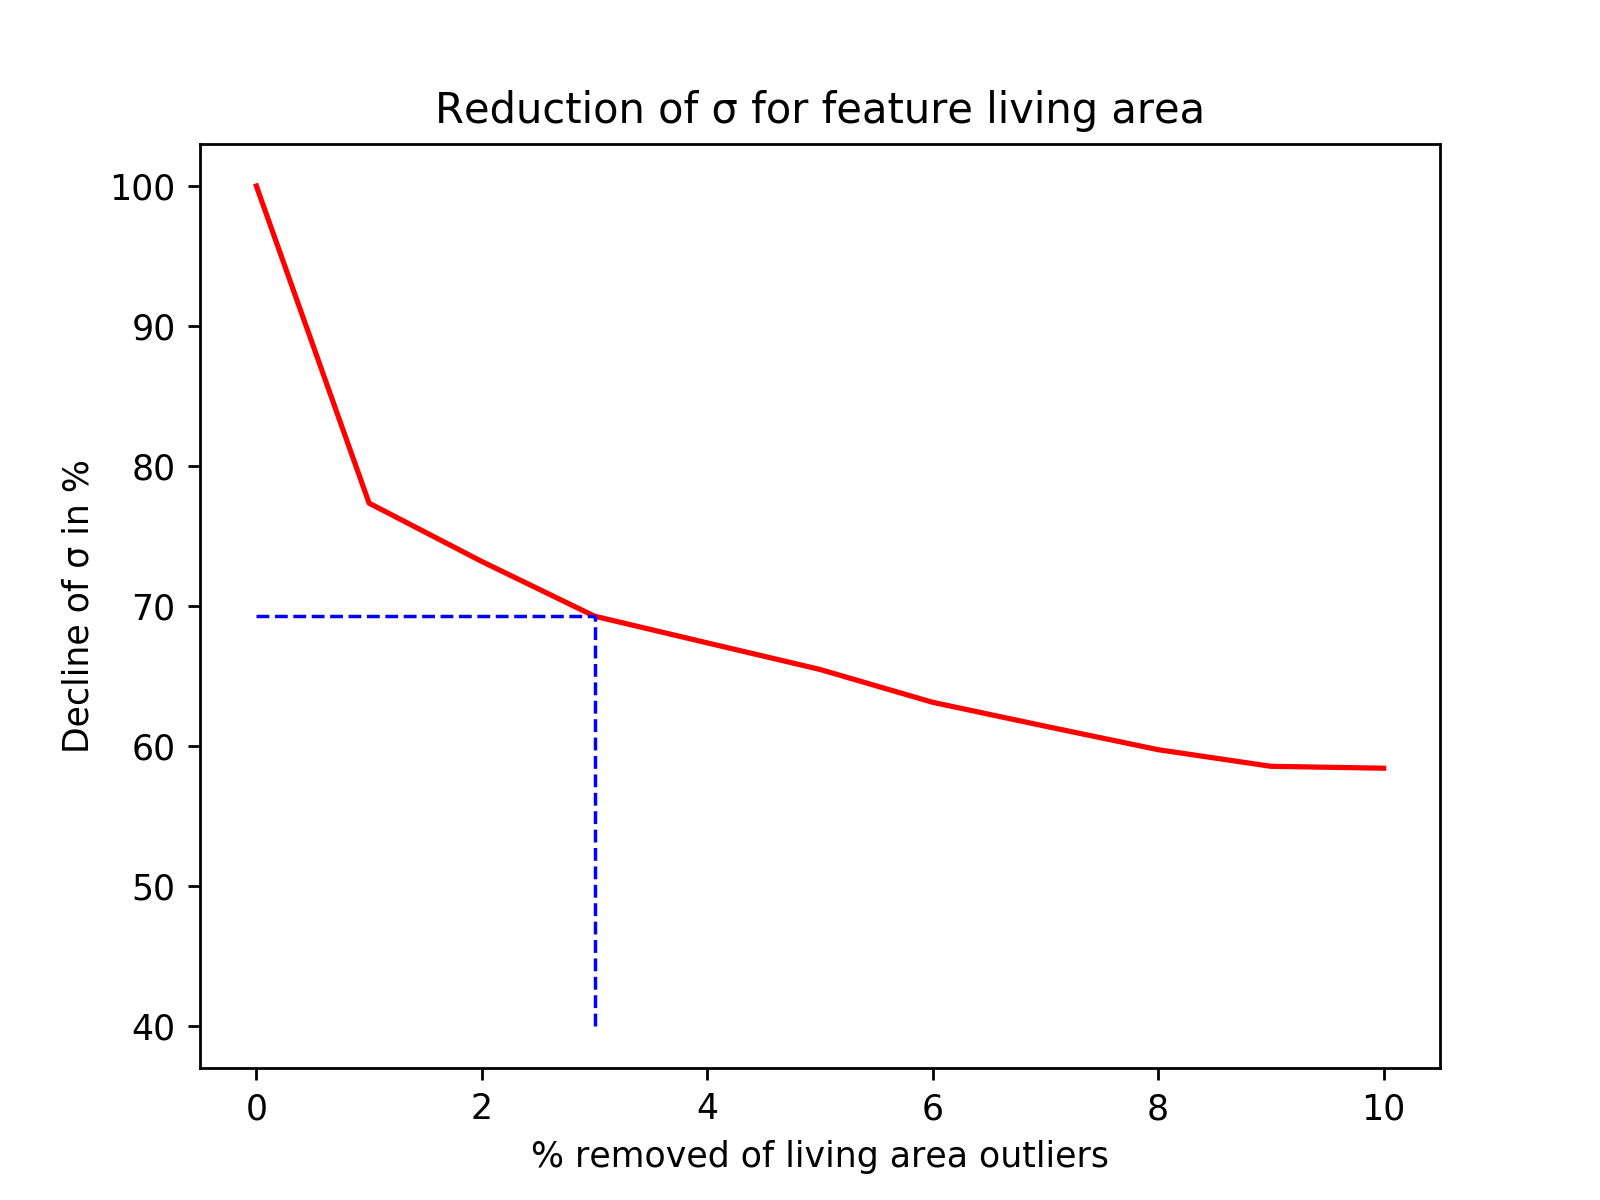
\includegraphics[width=\linewidth]{images/living_area_std.png}
  \caption[Entwicklung der Standardabweichung]{Entwicklung der Standardabweichung}
  \label{fig:isolation_std}
\end{subfigure}
\caption[Outlier Detection: Wohnfläche]{Outlier Detection: Wohnfläche}
\label{fig:outlier}
\end{figure}
%
Die Outlier Detection wird nach dem Transformieren der Features ausgeführt. Tabelle \ref{tab:iso_forest} zeigt die gefunden Ausreisser im Datensatz. Insgesamt wurden 12'362 Inserate als Ausreisser markiert und entfernt.\\[2ex]
%
\begin{table*}[ht]
\centering
\ra{1.3}
\begin{tabular}{@{}lrr@{}}
\toprule
Feature & Entfernt in \% & \# entfernte Inserate\\
\midrule
Baujahr & 5 & 4293\\
Anzahl Zimmer & 3 & 2579\\
Wohnfläche & 3 & 2577\\
Letzte Konstruktion & 5 & 4294\\
Lärmbelastung & 7 & 7726\\
\bottomrule
\end{tabular}
\caption{Übersicht der entfernten Inserate mit dem Isolation Forest}
\label{tab:iso_forest}
\end{table*}
%
Es ist unschwer zu erkennen, dass gewisse Inserate nicht nur bei einem Feature als Ausreisser markiert werden, sondern gleich bei mehreren.\\[2ex]
%
Betrachtet man die Einführung der Outlier Detection auf die Performance der Algorithmen in Tabelle \ref{tab:fifth_round}, sieht man, dass der Maximale Fehler auf 2 Millionen verkleinert wurde.\\
%
\begin{table*}[ht]
\centering
\ra{1.3}
\resizebox{\textwidth}{!}{
\begin{tabular}{@{}lrrrrr@{}}
\toprule
ML Algorithmus & $R^2$ & MAPE & MdAPE & 10\% Abweichung & Maximaler Fehler\\
\midrule
Extra Trees & 0.947074 & 5.216 & 0.702 & 84.269 & 1.89E+06\\
XGBoost & 0.941227 & 5.392 & 0.604 & 84.208 & 1.95E+06\\
AdaBoost &0.940529 & 4.692 & 0 & 85.609 & 1.95E+06\\
\bottomrule
\end{tabular}}
\caption{Ergebnisse mit Einbezug einer Outlier Detection}
\label{tab:fifth_round}
\end{table*}
%
Neben dem maximalen Fehler konnte auch die MAPE sowie auch die MdAPE verkleinert werden. Das zeigt die Wichtigkeit einer Outliner Detection. So trainieren die Modelle nicht an speziellen Daten.\\[2ex] 
%
Interessant zu wissen, wäre ob der Steuersatz eine Auswirkung auf das Modell hat. Deshalb haben wir vom Bundesamt für Statistik der Gemeinde- wie auch der Kontonssteuerfuss beschaffen und diesen in unser Modell miteinbezogen. Tablle \ref{tab:sixth_round} zeigt das Ergebnis.\\[2ex]
\begin{table*}[ht]
\centering
\ra{1.3}
\resizebox{\textwidth}{!}{
\begin{tabular}{@{}lrrrrr@{}}
\toprule
ML Algorithmus & $R^2$ & MAPE & MdAPE & 10\% Abweichung & Maximaler Fehler\\
\midrule
Extra Trees & 0.946107 & 5.39 & 0.686 & 83.799 & 1.55E+06\\
XGBoost & 0.940157 & 5.382 & 0.632 & 83.997 & 1.82E+06\\
AdaBoost &0.943958 & 4.64 & 0 & 85.596 & 1.81e+06\\
\bottomrule
\end{tabular}}
\caption{Ergebnisse mit Einbezug des Steuerfuss}
\label{tab:sixth_round}
\end{table*}
%
Es zeigt sich weder eine Verbesserung noch eine verschlechterung mit diesen beiden Features. Der Steuerfuss besittz demnach keinen grossen Einfluss auf den Immobilienpreis, beziehungsweise auf die Schätzungsmodelle.\\[2ex]
%
Unser Modell besitzt insgesamt 42 verschiedene Tags als Feature. Diese Tags beschreiben zum Teil dasselbe mit anderen Worten. Daher lohnt es sich aus mehreren schwachen Features ein starkes Feature zu bilden. Wir definieren 4 Gruppen die den Wert 1 besitzen, sobald ein Tag das zur Gruppe gehört vorhanden ist. Ansonsten ist es auf 0.
\begin{description}
\item[Badezimmer:] Alle Tags die eine Nasszelle beschreiben. Dazugehört Badezimmer, Lavabo, Dusche usw.
\item[Innenausstattung:] Alle Tags die eine Innenausstattung beschreiben wie TV Anschluss, gross, hell usw. 
\item[Aussenausstattung:] In diese Kategorie fallen Tags wie Garten, Balkon, Garage, Parkplatz usw.
\item[Nachbarschaft:] Beschreibt die Umgebung der Immobilie. Ist es zentral, ruhig, hat es Einkaufsmöglichkeiten usw.
\end{description}
%
Die Ergebnisse in Tabelle \ref{tab:seventh_round} zeigen nochmals eine Verbesserung der Modelle.\\ 
\begin{table*}[ht]
\centering
\ra{1.3}
\resizebox{\textwidth}{!}{
\begin{tabular}{@{}lrrrrr@{}}
\toprule
ML Algorithmus & $R^2$ & MAPE & MdAPE & 10\% Abweichung & Maximaler Fehler\\
\midrule
Extra Trees & 0.947874 & 4.854 & 0.109 & 85.541 & 2.54E+06\\
XGBoost &0.945822 & 4.881 & 0.074 & 85.759 & 2.50E+06\\
AdaBoost &0.93973 & 4.544 & 0 & 86.317 & 2.60E+06\\
\bottomrule
\end{tabular}}
\caption{Ergebnisse mit gruppierten Tags}
\label{tab:seventh_round}
\end{table*}
%
Mit unserem Feature Engineering konnten wir aufzeigen, dass eine deutliche Verbesserung der Modelle erreicht werden kann. Jetzt gilt es noch zu untersuchen, wie viel die ortsbezogenen Daten ausmachen. Dafür nehmen wir alle Features, die wir vom BFS gesammelt haben, aus unserer Featureliste und vergleichen das Resultat.\\
%
\begin{table*}[ht]
\centering
\ra{1.3}
\resizebox{\textwidth}{!}{
\begin{tabular}{@{}lrrrrr@{}}
\toprule
ML Algorithmus & $R^2$ & MAPE & MdAPE & 10\% Abweichung & Maximaler Fehler\\
\midrule
Extra Trees & 0.907327 & 7.092 & 0.684 & 79.063 & 1.96E+06\\
XGBoost & 0.892067 & 8.692 & 0.941 & 78.207 & 2.16E+06\\
AdaBoost & 0.893971 & 7.054 & 0 & 80.176 & 1.96E+06\\
\bottomrule
\end{tabular}}
\caption{Ergebnisse ohne ortsbezogenen Daten vom BFS}
\label{tab:height_round}
\end{table*}
%
Es ist in Tabelle \ref{tab:height_round} klar ersichtlich, dass ohne ortsbezogene Daten ein schlechteres Modell erstellt wird.

\subsubsection{Kombinierte Algorithmen}
Als weiteren Test haben wir einen eigenen Regressor erstellt, der mehrere Machine Learnig Algorithmen kombiniert.\\[2ex]
%
Dieser Algorithmus hat im Endeffekt zwei Schätzphasen. Zunächst wird ein Extra Trees trainiert, und für jeden Train-Datensatz werden alle Decision Pathes für alle Bäume abgespeichert. Um nun eine Schätzung zu erhalten, werden zuerst die Decision Pathes für den zu testenden Datensatz herausgesucht, und mit den Train-Datensätzen verglichen. Alle Train-Datensätze mit mindestens einem passendem Decision Path werden markiert für die zweite Phase der Schätzung.\\
In der zweiten Phase werden diese markierten Datensätze auf einem weiteren Machine Learning Algorithmus ad-hoc trainiert. Der zweite Algorithmus kann nach beliben ausgetauscht werden. Anschliessend wird auf diesem neuen Model der Test-Datensatz geschätzt.\\
Theoretisch wäre es möglich für alle möglichen Decision Pathes die Models im Vorhinein zu berechnen, da nur eine finite Anzahl an Decision Pathes existieren. Dies ist aber aus praktikablen Gründen nicht möglich, da mit vielen Datensätzen die trainierten Bäume gross werden und entsprechend  dafür zu viel RAM und Rechenzeit benötigt wird.\\[2ex]
%
Um genügend Datensätze für die zweite Phase zu erhalten, wird der Extra Trees mit einer minimalen Leaf Size von fünf Samples konfiguriert.\\
Für den zweiten Schätzungsalgorithmus verwenden wir den K-Nearest Neighbour wie oben beschrieben.
%
\begin{table*}[ht]
\centering
\ra{1.3}
\resizebox{\textwidth}{!}{
\begin{tabular}{@{}lrrrrr@{}}
\toprule
ML Algorithmus & $R^2$ & MAPE & MdAPE & 10\% Abweichung & Maximaler Fehler\\
\midrule
Extra Trees mit KNN & 43.636 & 13.451 & 40.034 &  0.619114 & 2.94294e+07\\
\bottomrule
\end{tabular}}
\caption{Ergebnisse ohne ortsbezogenen Daten vom BFS}
\label{tab:combined}
\end{table*}
%
Wie man in Tabelle \ref{tab:combined} sieht, waren die Ergebnisse weitaus schlechter als oben verwendete Algorithmen. Wir können uns dieses Verhalten nicht erklären. Weitere Forschungen konnten nicht durchgeführt werden, da uns für das die Zeit fehlte.\\[2ex]
%
Als letztes kombinieren wir noch die drei Baumalgorithmen miteinander. Da der AdaBoost immer ein bisschen besser war als die anderen beiden, erhält dieser mehr Gewicht für die Schätzung. Das Resultat konnte nochmals verbessert werden, wie Tabelle \ref{tab:combined_2} angezeigt.\\
Hierfür wurden dem AdaBoost 0.8, dem XGBoost 0.2 und dem Extra Trees 0.1  Gewichtung gegeben.
%
\begin{table*}[ht]
\centering
\ra{1.3}
\resizebox{\textwidth}{!}{
\begin{tabular}{@{}lrrrrr@{}}
\toprule
ML Algorithmus & $R^2$ & MAPE & MdAPE & 10\% Abweichung & Maximaler Fehler\\
\midrule
Kombiniert & 0.94646 & 4.416 & 0.07 & 87.03	& 1.77E+06\\
\bottomrule
\end{tabular}}
\caption{Ergebnisse ohne ortsbezogenen Daten vom BFS}
\label{tab:combined_2}
\end{table*}

%
\subsection{Auswertung}
Es hat sich gezeigt, dass eine Kombination des AdaBoost, Extra Trees und XGBoost die besten Resultate erzielt. Betrachtet man die Algorithmen alleine hatte bei unseren Daten der AdaBoost die besten Ergebnisse.\\ 
Von der Berechnungszeit ist der AdaBoost klar der Beste, da dieser für ein Fit ungefähr 10 Minuten benötigt, während er XGBoost under der Extra Trees über eine Stunde benötigen.\\
Wir konnten mit unserer eigenen Implementation eines Machine Learning Algorithmus keinen Erfolg erzielen, da die Performance nicht zufriedenstellend war.\\[2ex]
%
Weiter konnte bewiesen werden, dass sich ein ausgiebiges Feature Engineering auf die Performance positiv auswirkt. Vor allem eine Outlier Detection kann das Modell um 10\% verbessern. Der Versuch seltene Features so zu transformieren, dass man sie verwenden kann, hilft auch um eine bessere Performance zu erhalten. \\
Es ist Sinnvoll ortsbezogene Daten als Features zu verwenden. Mit diesen Features konnte eine Steigerung von 4\% bei den richtig Geschätzten Immobilien erzielt werden. Das zeigt, dass der Preis nicht nur von der Immobilie sondern auch vom Standort abhängig ist. \\[2ex]
%
Auch wenn die öffentlichen Daten von Immobilien eine eher schlechte Qualität besitzen, reichen sie aus für ein gutes Schätzungsmodell. Insgesamt konnten 85’845 von 162’225 verwendet werden. Die meisten Inserate konnten nicht verwendet werden, da sie keine Angaben über wichtige Kennwerte hatten.

subsection{Gültigkeitsrisiken}
Man muss bedenken, dass wir unsere Modelle auf geschätzten Werten trainiert haben. Somit ist der geschätzte Wert mit Vorsicht zu betrachten. Auch ist der Immobilienpreis immer gewissen Schwankungen ausgesetzt sodass dieser in einem halben Jahr schon wieder anderst ist.\\
Wir haben die Kennwerte von öffentlichen Immobilienplattformen gesammelt. Es geht dort hauptsächlich darum die Immobilie zu verkaufen. So wird auch gerne mal ein bisschen geschummelt, schöngeredet oder die Angaben der Kennwerte werden falsch eingetragen. Eine Outlier Detection kann nur grobe Ausreisser erkennen. Kleinere Ausreisser bleiben somit unentdeckt und können das Modell verfälschen.\\
Wird eine neue Siedlung oder ein neuer Wohnblock inseriert, kann es vorkommen, dass 10 mal die gleiche Wohnung inseriert wird. Dies ist unschön, da diese Wohnungen mehr Gewicht erhalten.

